\chapter{L5 - Paging}
\textit{Fellow syscoms, this is yet another chapter that was already studied in computer architecture, however, don't be discouraged, I'll do my best to make things clear. Again, please send me a text if anything lacks clarity, with that said, good luck.}\\[5px]
\textit{For context, we've established that a specialized hardware was required to efficiently translate virtual addresses into physical addresses. However, this introduces another critical requirement: optimizing memory usage. To address this, paging becomes essential, enabling dynamic memory allocation and effectively managing address space constraints.}
\vfill
\section{Page-based Memory Management Unit (MMU)}
In modern operating systems, paging is used to manage memory efficiently by dividing both the virtual address space and physical memory into fixed-size blocks. This section provides a detailed overview of how paging works and how addresses are translated.

\subsection{Overview of Paging}
\textit{Personal Remark:} Although the physical frames allocated to a process may be non-contiguous, the virtual address space appears contiguous to the process.\\
\noindent
\begin{minipage}{0.45\textwidth}
  \begin{itemize}
    \item[-] \textbf{Pages:} Fixed-size blocks that partition the virtual address space.
  \item[-] \textbf{Frames:} Fixed-size blocks that partition physical memory.
  \item[-] \textbf{Mapping:} Each page is associated with a frame via a mapping (i.e., \{page $\rightarrow$ frame\}). This allows the operating system to apply protection at the page level.
\end{itemize}
\end{minipage}
\hfill
\vline
\hfill
\begin{minipage}{0.45\textwidth}
\begin{center}
  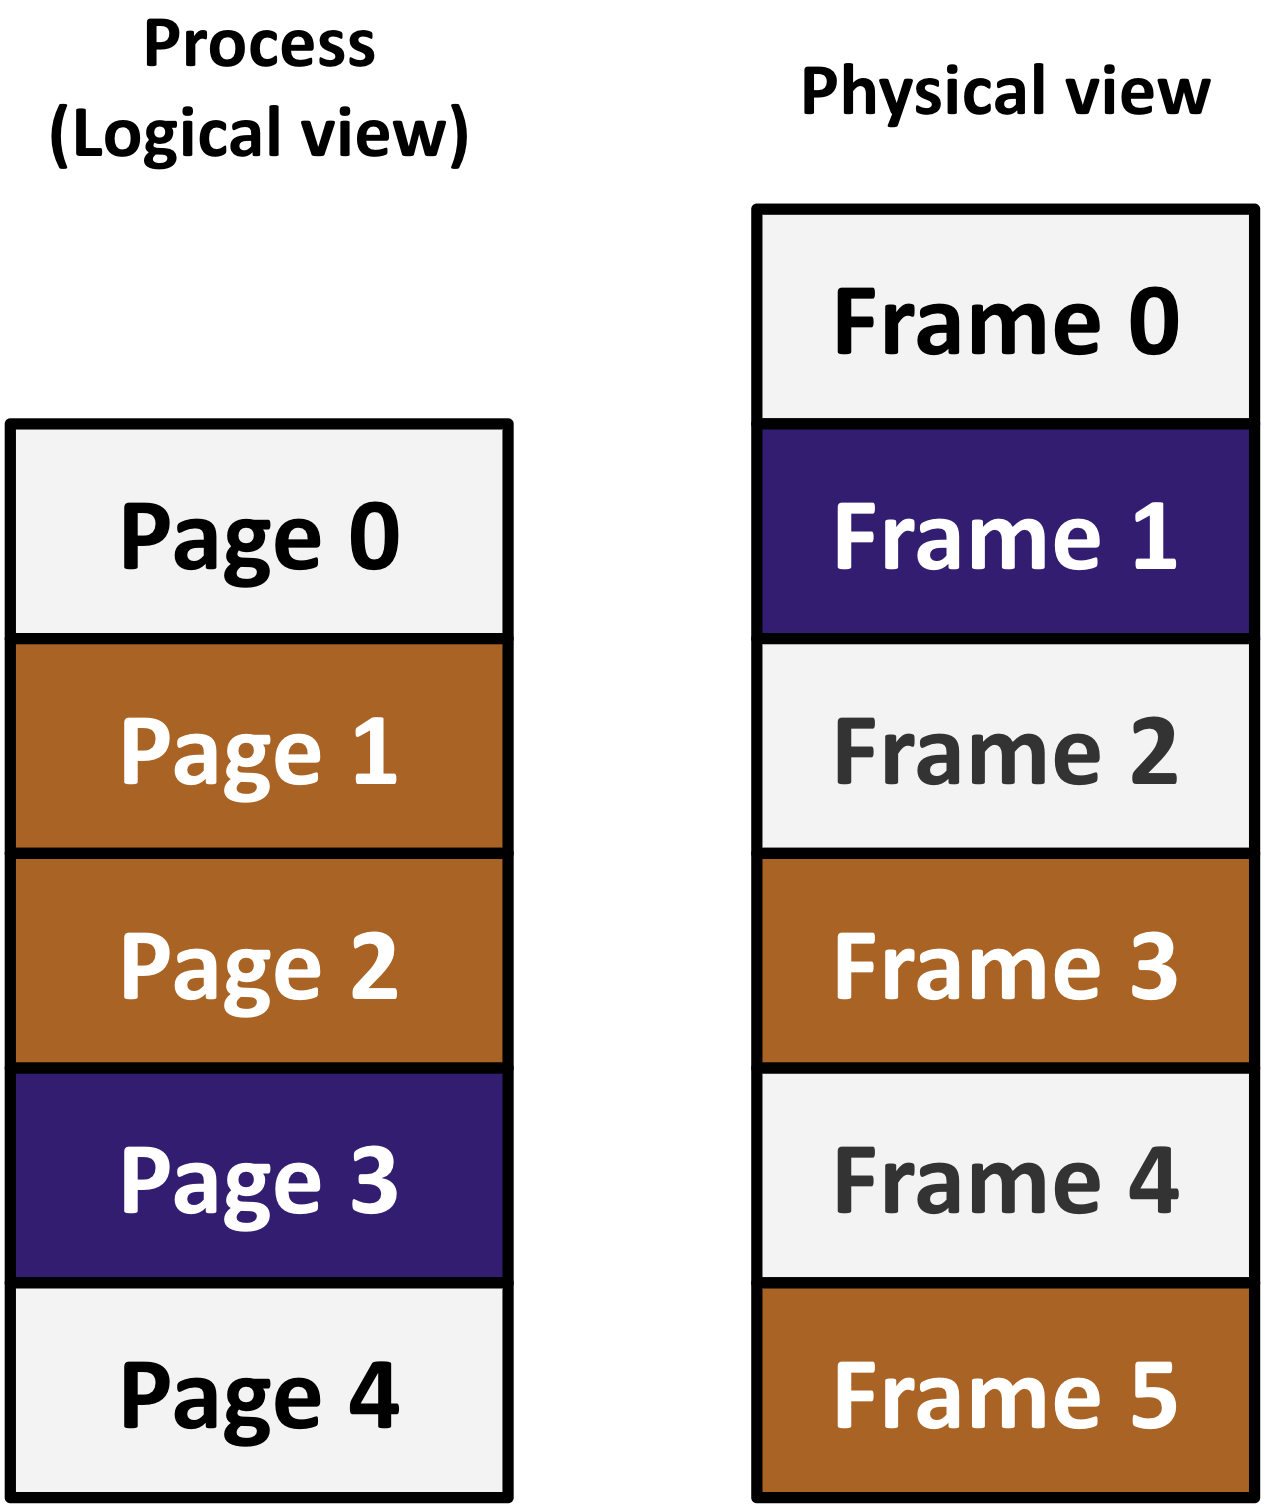
\includegraphics[width=0.6\textwidth]{chapters/L5/images/page-mmu.png}
\end{center}
\end{minipage}\\
\newpage
\subsection{Size of a Page}
A page is the smallest unit of memory allocation in a paging system. Its size is chosen based on the following considerations:\\
\noindent
\begin{minipage}{0.45\textwidth}
\begin{itemize}
  \item[-] \textbf{Minimizing Internal Fragmentation:} Typical page sizes range from 4 KB to 16 KB.
  \item[-] \textbf{Management Overhead:} Smaller pages lead to larger page tables, while larger pages can waste memory.
\end{itemize}

\textbf{Super Pages:} These are larger blocks made up of multiple contiguous pages (e.g., 2 MB or 1 GB). They reduce the overhead associated with page translation. \\
\end{minipage}%
\hfill
\vline
\hfill
\begin{minipage}{0.45\textwidth}
\begin{center}
  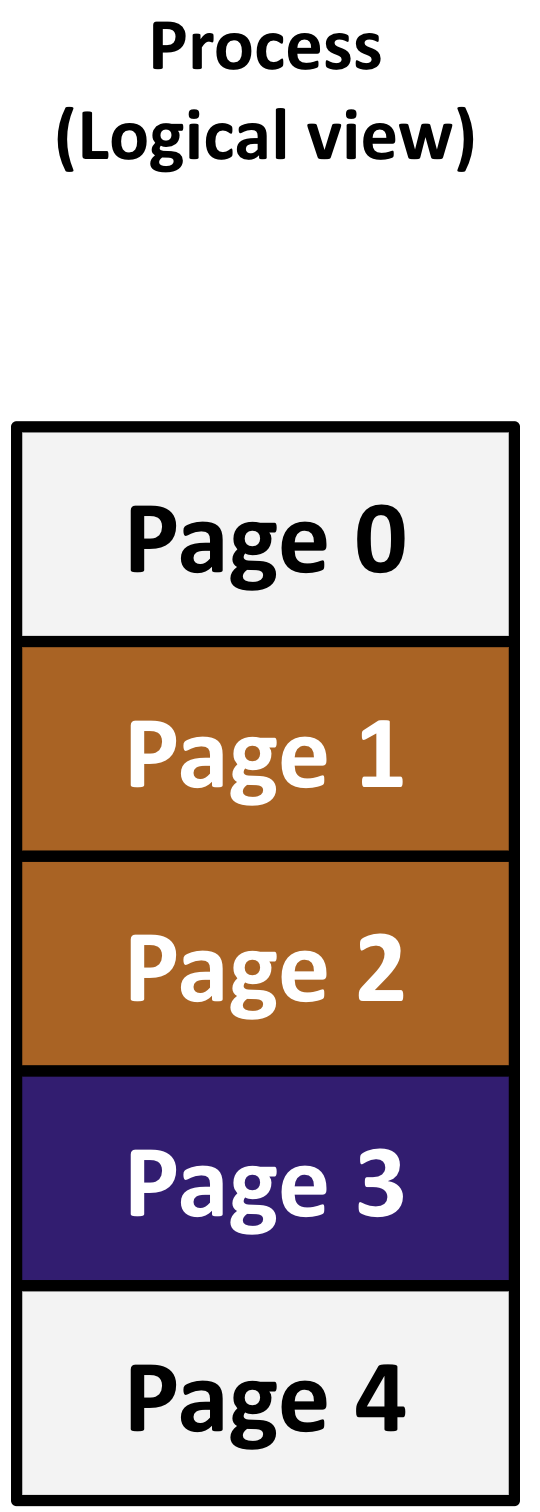
\includegraphics[width=0.35\textwidth]{chapters/L5/images/page-size.png}
\end{center}
\end{minipage}\\

\subsection{Memory Management Scheme}
The operating system manages memory using the following scheme:\\[5px]
\noindent
\begin{minipage}{0.45\textwidth}
\begin{enumerate}
  \item \textbf{Frame Allocation:} Logical pages are mapped to available physical frames based on the OS's allocation strategy.
  \item \textbf{Page Table:} The OS maintains a data structure called the page table, which stores the mapping between logical pages and physical frames.
  \item \textbf{Per-Process Management:} Each process has its own page table to manage its virtual address space.
\end{enumerate}
\end{minipage}%
\hfill
\vline
\hfill
\begin{minipage}{0.45\textwidth}
  \begin{center}
    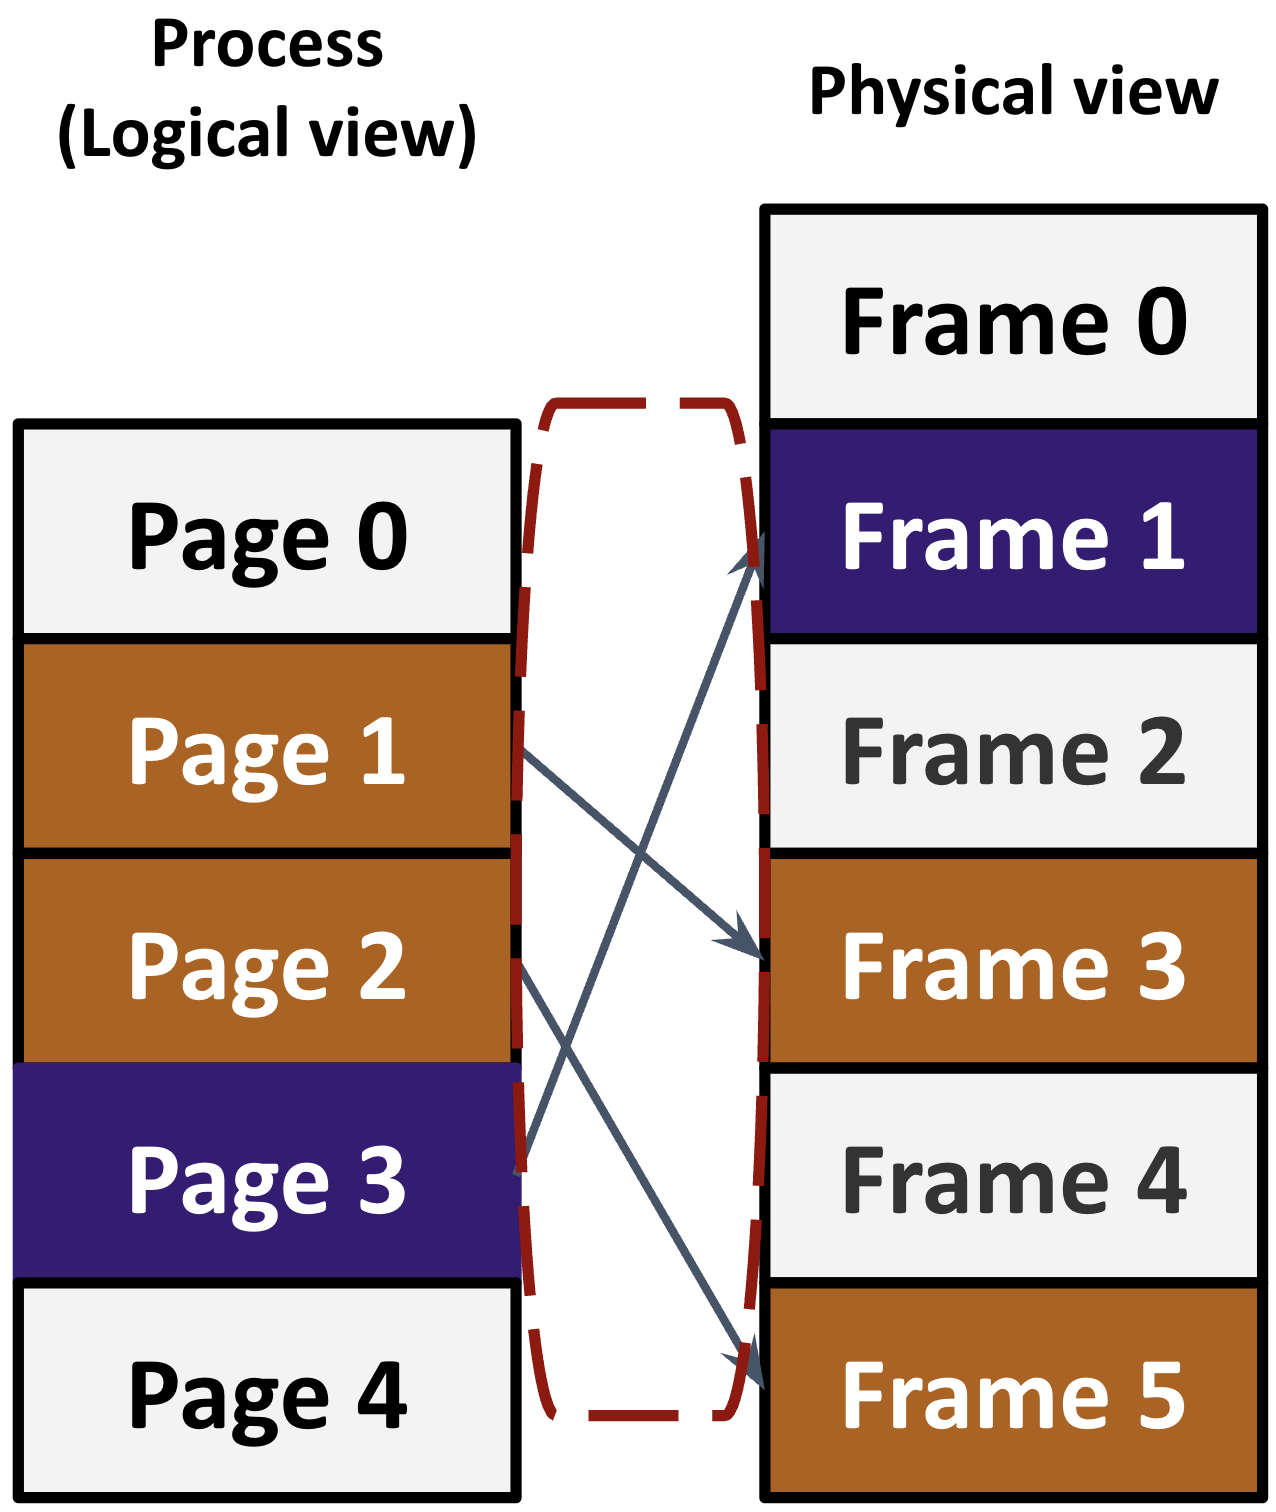
\includegraphics[width=0.45\textwidth]{chapters/L5/images/mapping.png}
  \end{center}
\end{minipage}

\subsection{Address Representation}
A virtual address is composed of two distinct components:
\begin{enumerate}
  \item \textbf{Virtual Page Number (VPN):} The higher-order \textit{p} bits of the address that identify the page in the virtual address space.
  \item \textbf{Page Offset:} The lower-order \textit{o} bits that specify the exact byte within the page.
\end{enumerate}

\begin{minipage}{\linewidth}
  \centering
  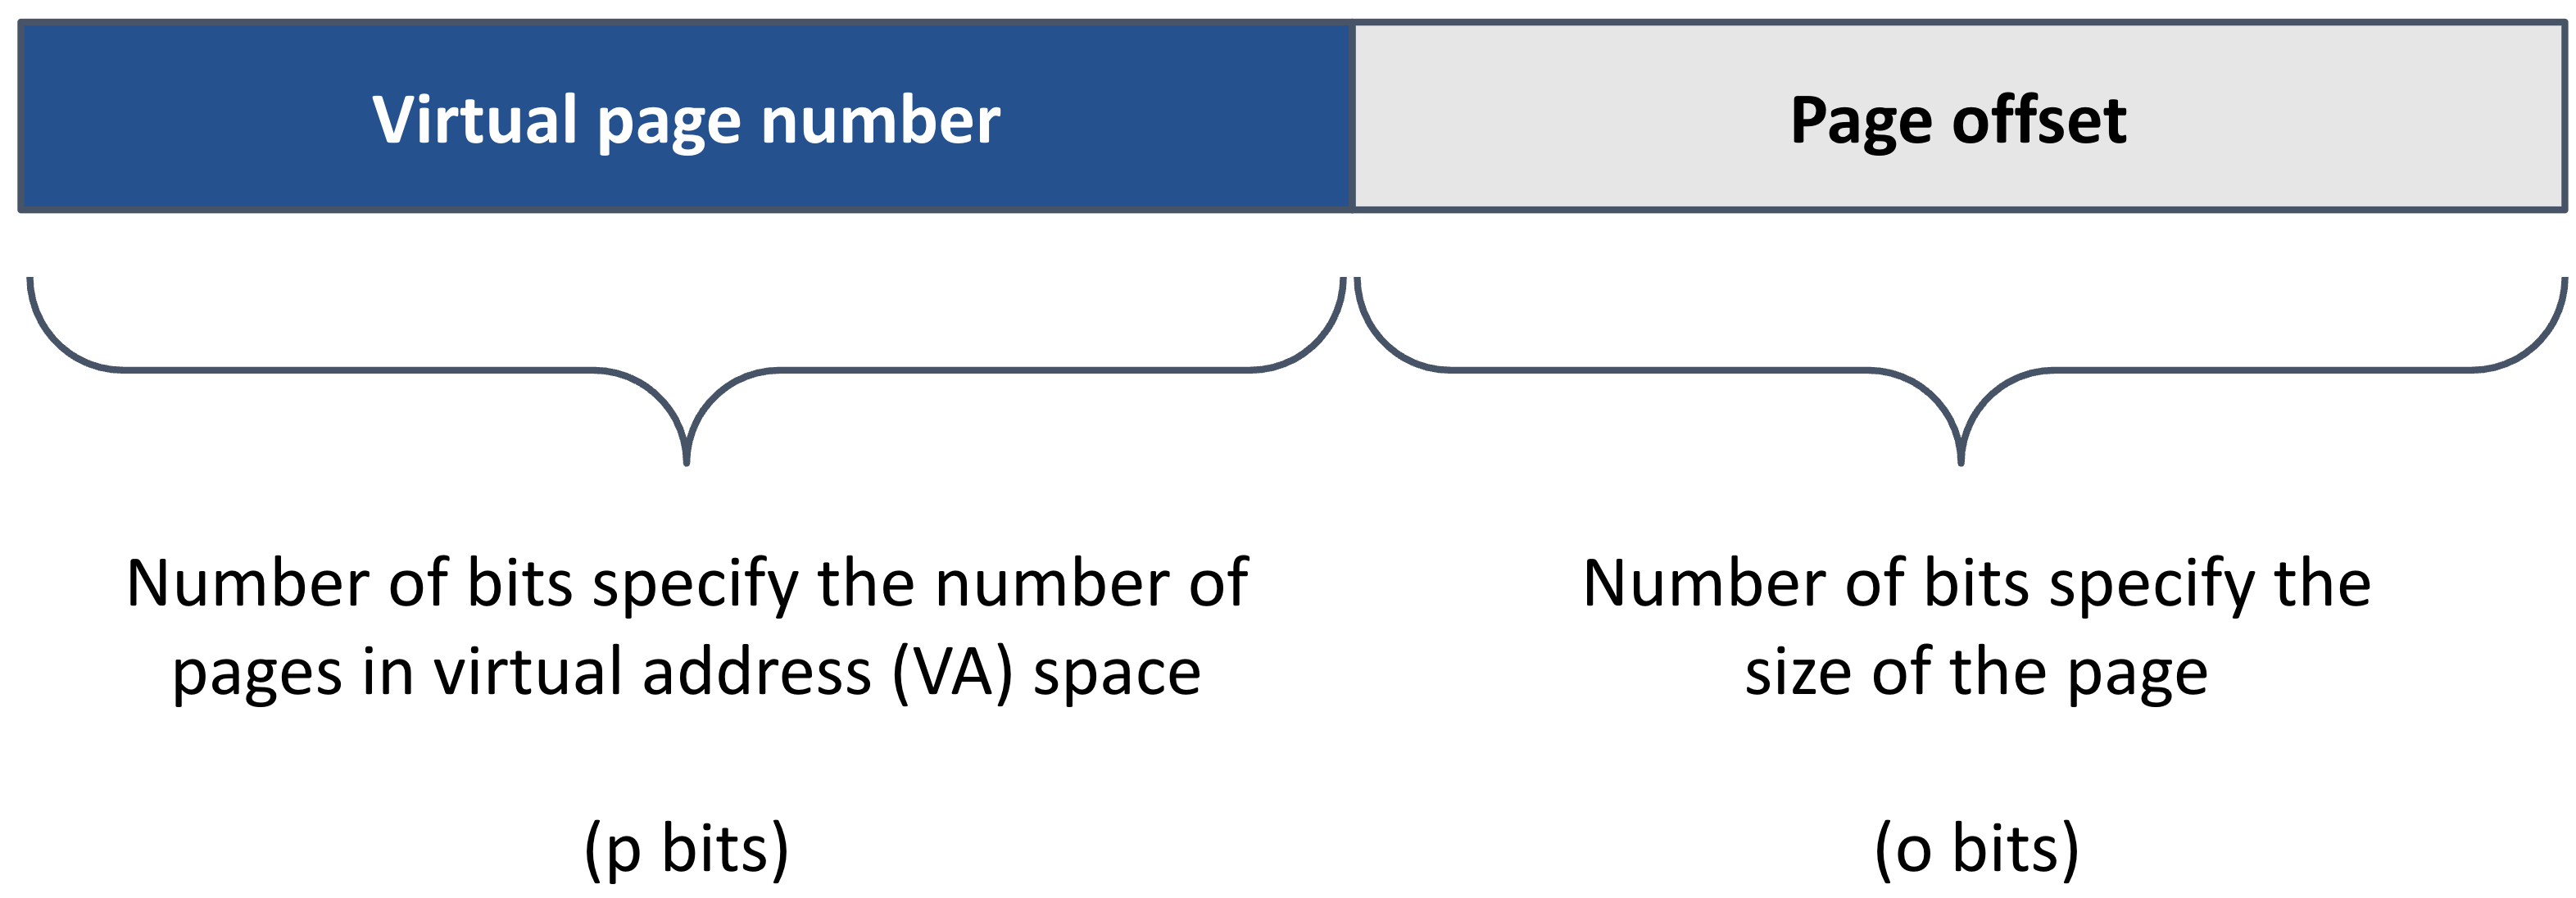
\includegraphics[width=0.65\textwidth]{chapters/L5/images/virtual.png}
\end{minipage}
\newpage
\begin{example}[Virtual Address Example (32-bit Architecture)]
In a 32-bit system, the virtual address is divided into a virtual page number and a page offset, as illustrated below.\\
\begin{center}
  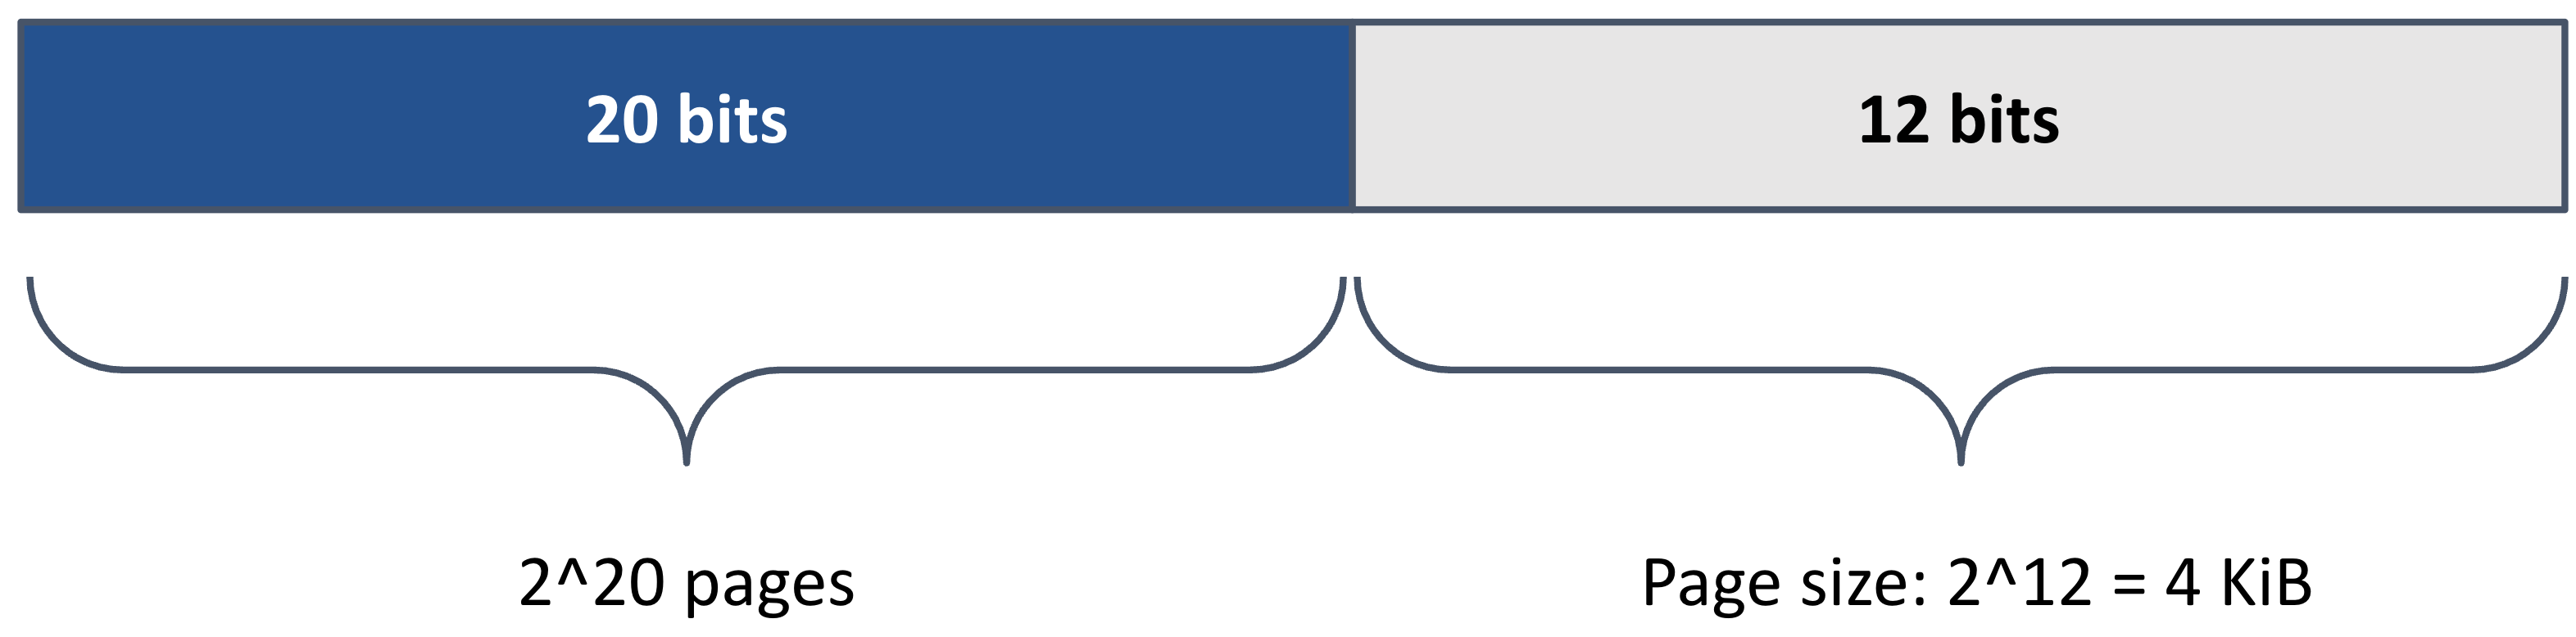
\includegraphics[width=0.65\textwidth]{chapters/L5/images/paging-example.png}
\end{center}
\end{example}

\subsection{Address Translation}
Address translation is the process by which the Memory Management Unit (MMU) converts a virtual address into a physical address. The steps involved are:
\begin{enumerate}
  \item \textbf{Extract the Virtual Page Number:} Take the first \textit{p} bits of the virtual address.
  \item \textbf{Map to Physical Frame:} Use the page table to find the corresponding physical frame number.
  \item \textbf{Extract the Page Offset:} Take the remaining \textit{o} bits.
  \item \textbf{Compute the Physical Address:} Combine the frame number with the offset to access the specific byte in physical memory.
\end{enumerate}

\begin{center}
  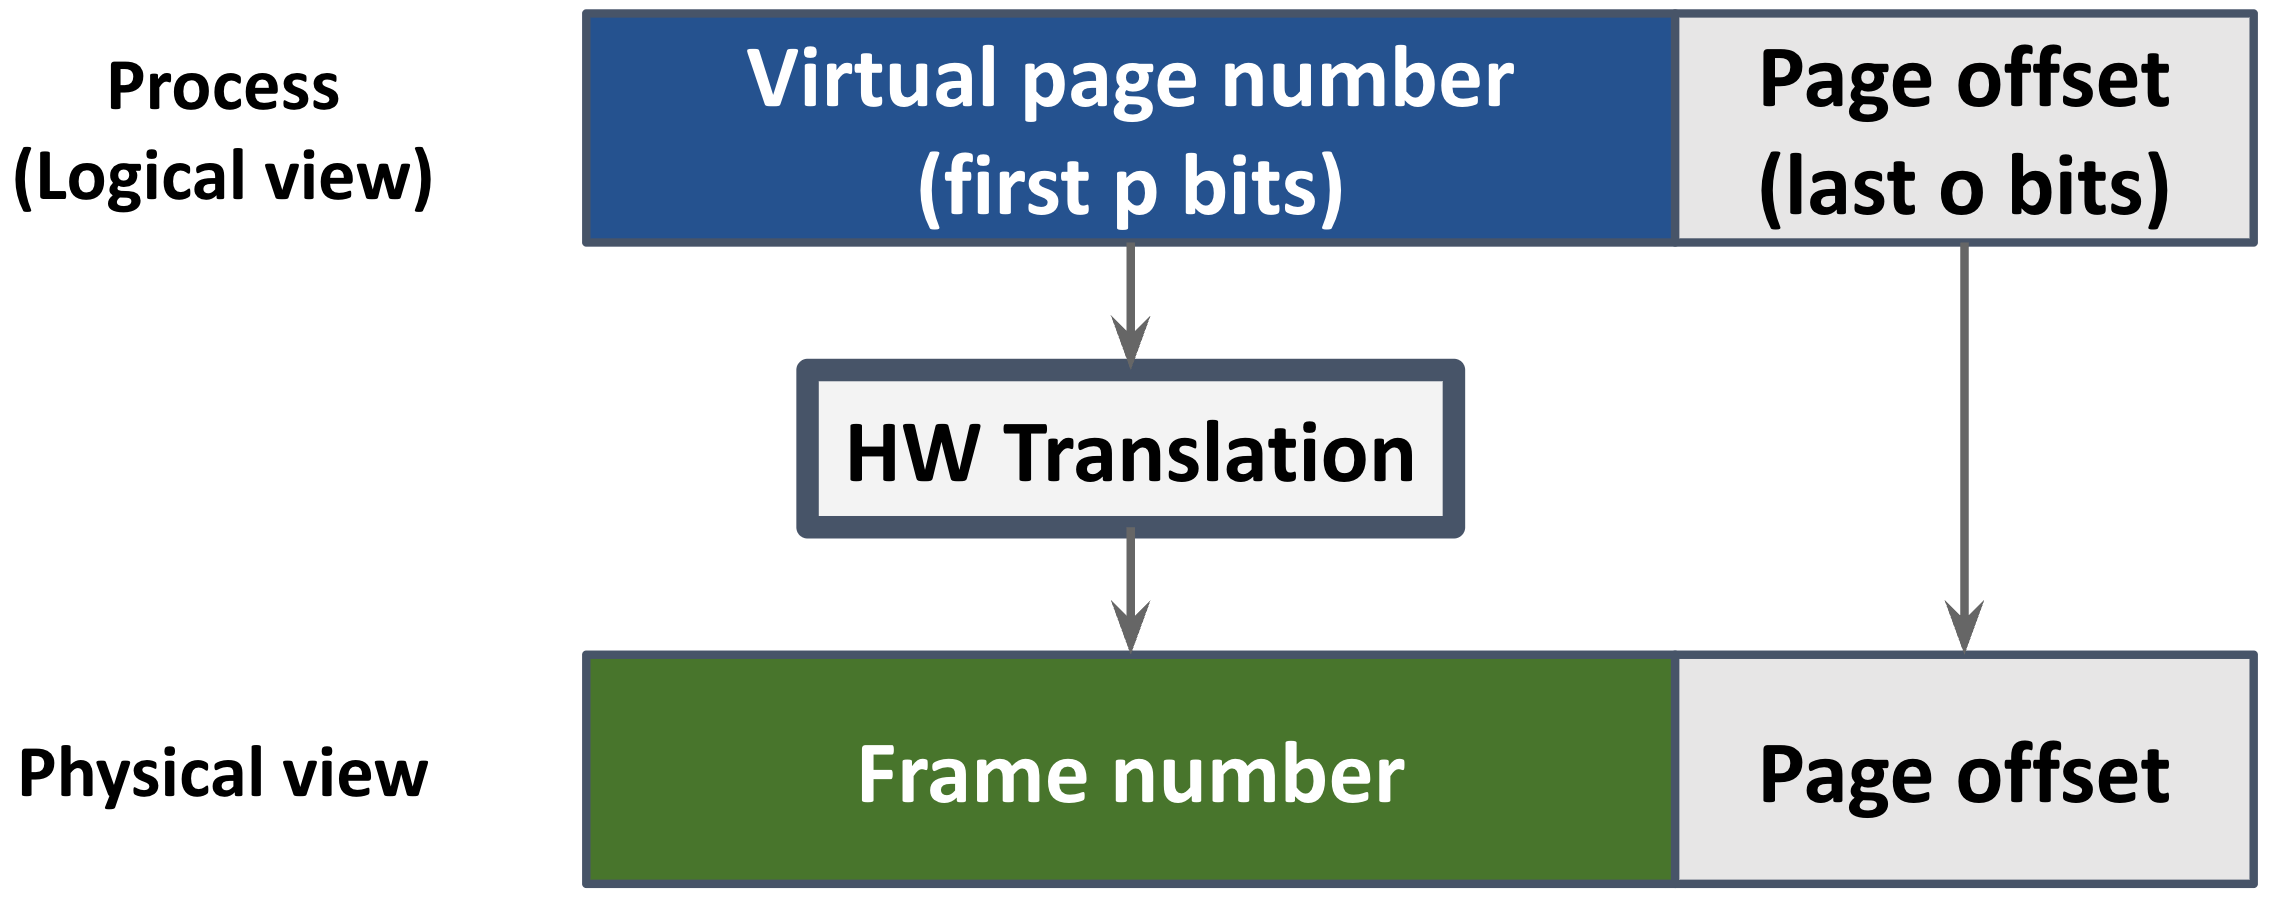
\includegraphics[width=0.45\textwidth]{chapters/L5/images/translation.png}
\end{center}

\vspace{40px}
\subsubsection{Accessing a Byte}
To access a specific byte in memory, the MMU follows these steps:
\begin{enumerate}
  \item Extract the virtual page number from the virtual address.
  \item Map this virtual page number to the corresponding physical frame using the page table.
  \item Extract the offset from the virtual address.
  \item Access the byte at the calculated physical memory location.
\end{enumerate}

\textit{Personal Remark:} This systematic approach to address translation is fundamental to the operation of virtual memory systems, ensuring efficient and secure memory access.

\newpage
\subsection{Virtual Address Space}
\begin{example}[Virtual Address Space]
\leavevmode\\
\noindent
\begin{minipage}{0.55\textwidth}
  Consider a virtual address space consisting of 64 bytes, divided into 4 fixed-size pages of 16 bytes each. Assume all components of a program (code, stack, heap) comfortably fit into this address space.\\[5px]
\textbf{Question:} What is the size of a pointer necessary to uniquely address any byte in this address space?\\
\textbf{Answer:} 6 bits, since $\log_2(64) = 6$ bits are needed to uniquely represent each byte.
\end{minipage}%
\hfill
\vline
\hfill
\begin{minipage}{0.35\textwidth}
\begin{center}
  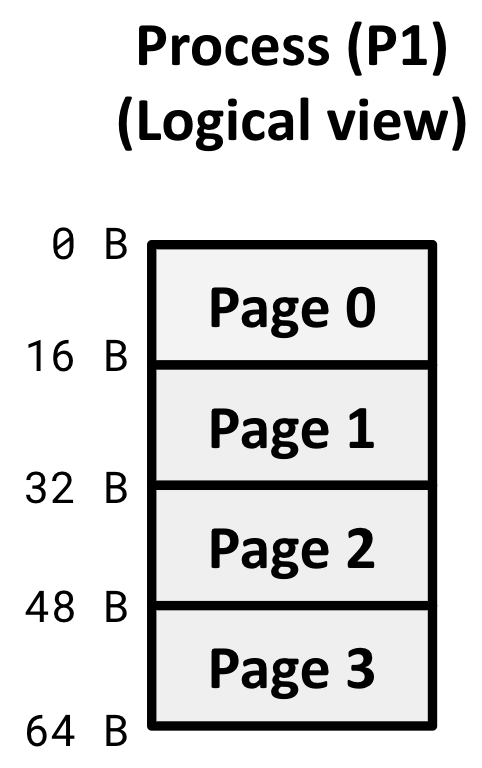
\includegraphics[width=0.45\textwidth]{chapters/L5/images/question.png}
\end{center}
\end{minipage}\\
\end{example}

\subsection{Physical Memory}

\begin{example}[Physical Memory]
\leavevmode
\\[2px]
Physical memory is composed of fixed-size storage slots called \textit{page frames}. Suppose there are 8 page frames, each 16 bytes, making the total physical memory 128 bytes. This setup requires at least 7 bits to uniquely represent any physical memory location ($\log_2(128) = 7$ bits). \\
\noindent
\begin{minipage}{0.45\textwidth}
The virtual pages of a process (e.g., process P1) map to physical memory frames as follows:\\

\begin{itemize}
  \item Virtual page 0 $\rightarrow$ Physical frame 3
  \item Virtual page 1 $\rightarrow$ Physical frame 7
  \item Virtual page 2 $\rightarrow$ Physical frame 5
  \item Virtual page 3 $\rightarrow$ Physical frame 2
\end{itemize}
\end{minipage}%
\hfill
\vline
\hfill
\begin{minipage}{0.45\textwidth}
\begin{center}
  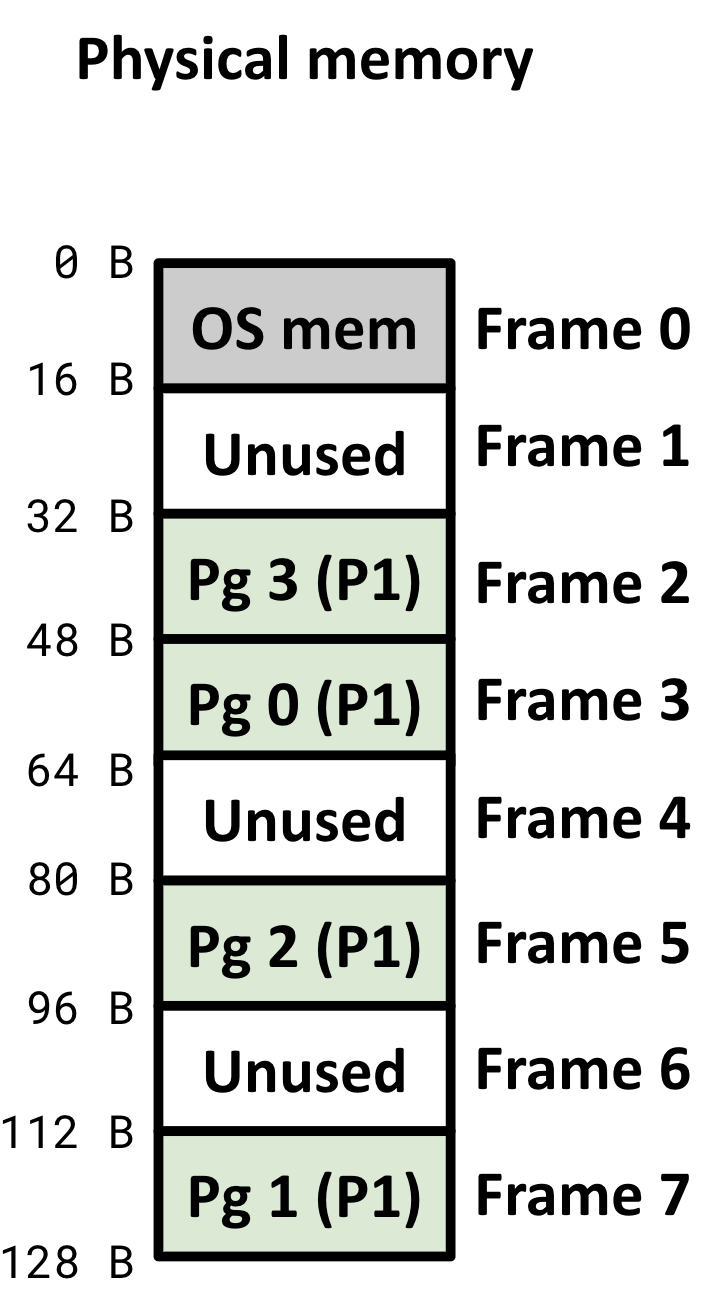
\includegraphics[width=0.45\textwidth]{chapters/L5/images/paging-example2.png}
\end{center}
\end{minipage}
\\

\end{example}

\subsection{Virtual Address Translation}

\begin{example}[Virtual Address Translation]
\leavevmode \\[2px]
\noindent
\begin{minipage}{0.45\textwidth}
Consider that process P1 attempts to access a memory location using the following assembly instruction:
\[
\texttt{movl 21, \%eax}
\]
This instruction moves 4 bytes starting from virtual address 21 into the \%eax register. However, the data does not physically reside at virtual address 21; instead, it is stored in physical memory. Specifically, virtual address 21 belongs to virtual page 1, which maps to physical frame 7:
\end{minipage}%
\hfill
\vline
\hfill
\begin{minipage}{0.45\textwidth}
\begin{center}
  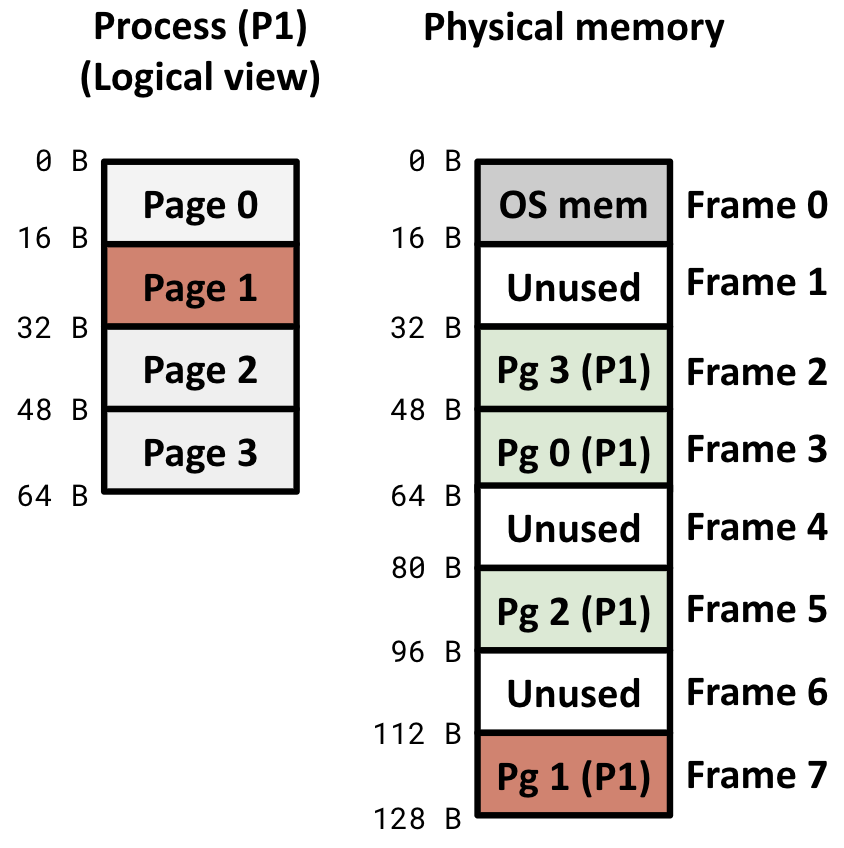
\includegraphics[width=0.9\textwidth]{chapters/L5/images/paging-example3.png}
\end{center}
\end{minipage}\\
\end{example}
\newpage
\begin{example}[Computing Virtual Page Number and Offset]
\leavevmode
\\[5px]
Given:
\begin{itemize}
  \item[-] Virtual address space: 64 bytes (6 bits)
  \item[-] Page size: 16 bytes (4 bits for offset)
\end{itemize}

Thus, the remaining $6 - 4 = 2$ bits represent the virtual page number.\\[5px]

\textbf{Question:} Determine the virtual page number and offset for the instruction \texttt{movl 21, \%eax}.

The binary representation of 21 is \texttt{010101}. Thus:
\begin{itemize}
  \item Virtual page number: first 2 bits (01) $\rightarrow$ Page 1
  \item Offset: last 4 bits (0101)
\end{itemize}

Given the page table mapping, virtual page 1 corresponds to physical frame 7 (binary \texttt{111}):

\begin{center}
  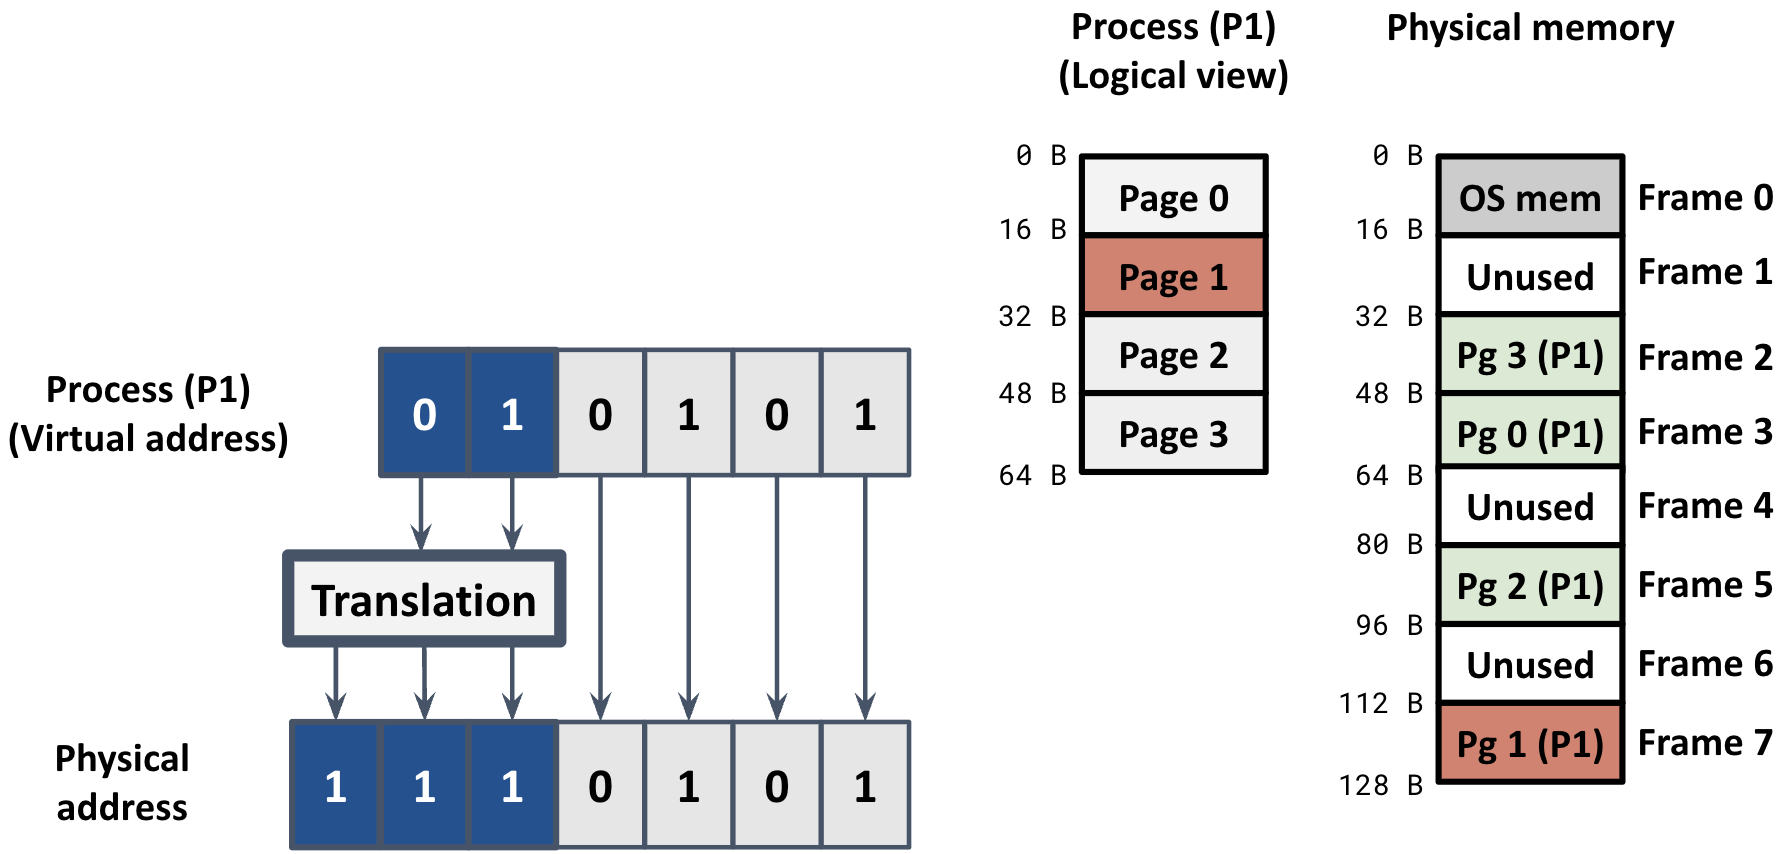
\includegraphics[width=0.85\textwidth]{chapters/L5/images/paging-example4.png}
\end{center}
\end{example}

\section{The Page Table}

\begin{definition}[Page Table]
\leavevmode
\\[2px]
A \textbf{page table} is a data structure maintained by the operating system that stores the mapping between virtual addresses and their corresponding physical addresses. Each process has its own dedicated page table.

The pointer to the currently active page table is stored in a special register known as the \textit{page-table base register} (PTBR). On x86 architectures, this register is typically referred to as \texttt{\%cr3}. During context switches, the operating system saves and restores the PTBR value from the process control block (PCB).
\end{definition}
\subsection{Structure of Page Table Entries}
The page table consists of multiple \textbf{page table entries} (PTEs). Each entry stores not only the \textit{page frame number} (PFN) that provides the mapping between virtual pages and physical frames but also additional status information. Important fields in a PTE typically include:

\begin{itemize}
  \item[-] \textbf{Present bit}: Indicates if the translation is valid and the page resides in physical memory.
  \item[-] \textbf{Protection bits}: Define access permissions (read, write, execute).
  \item[-] \textbf{User/Supervisor bit (U/S)}: Differentiates between user-mode and kernel-mode access permissions.
  \item[-] \textbf{Dirty bit}: Indicates if the page has been modified (written to).
  \item[-] \textbf{Access/Reference bit}: Used to track page usage patterns and inform page replacement algorithms.
\end{itemize}
\newpage
Below, the 32-bit Intel PTE format
\begin{center}
  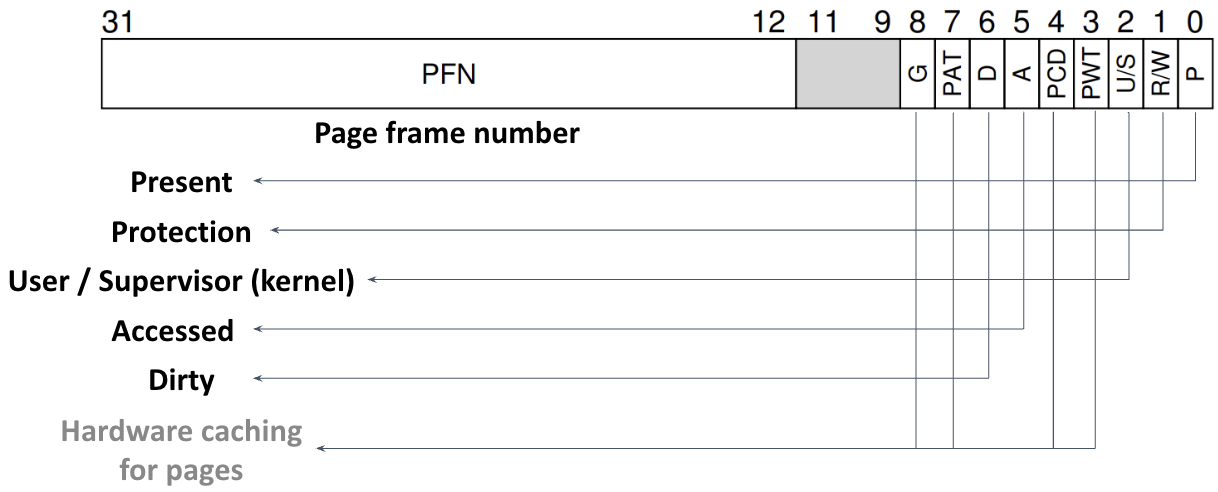
\includegraphics[width=0.85\textwidth]{chapters/L5/images/intel.png}
\end{center}

Additionally, each page table entry is always aligned to the page size for efficient access by the hardware.


\section{Organizing the Page Table Structure}

The simplest implementation is the \textbf{linear page table}. The Memory Management Unit (MMU) indexes directly into the page table using the \emph{virtual page number}.

The process involves the following steps:
\begin{enumerate}
    \item The MMU uses the virtual page number as an index into the linear array of page table entries.
    \item It retrieves the corresponding \emph{page table entry (PTE)} at this index.
    \item From the PTE, the MMU obtains the associated \emph{physical frame number}.
\end{enumerate}

A linear page table requires the allocation of multiple contiguous memory pages to store the entire mapping structure.

\begin{center}
  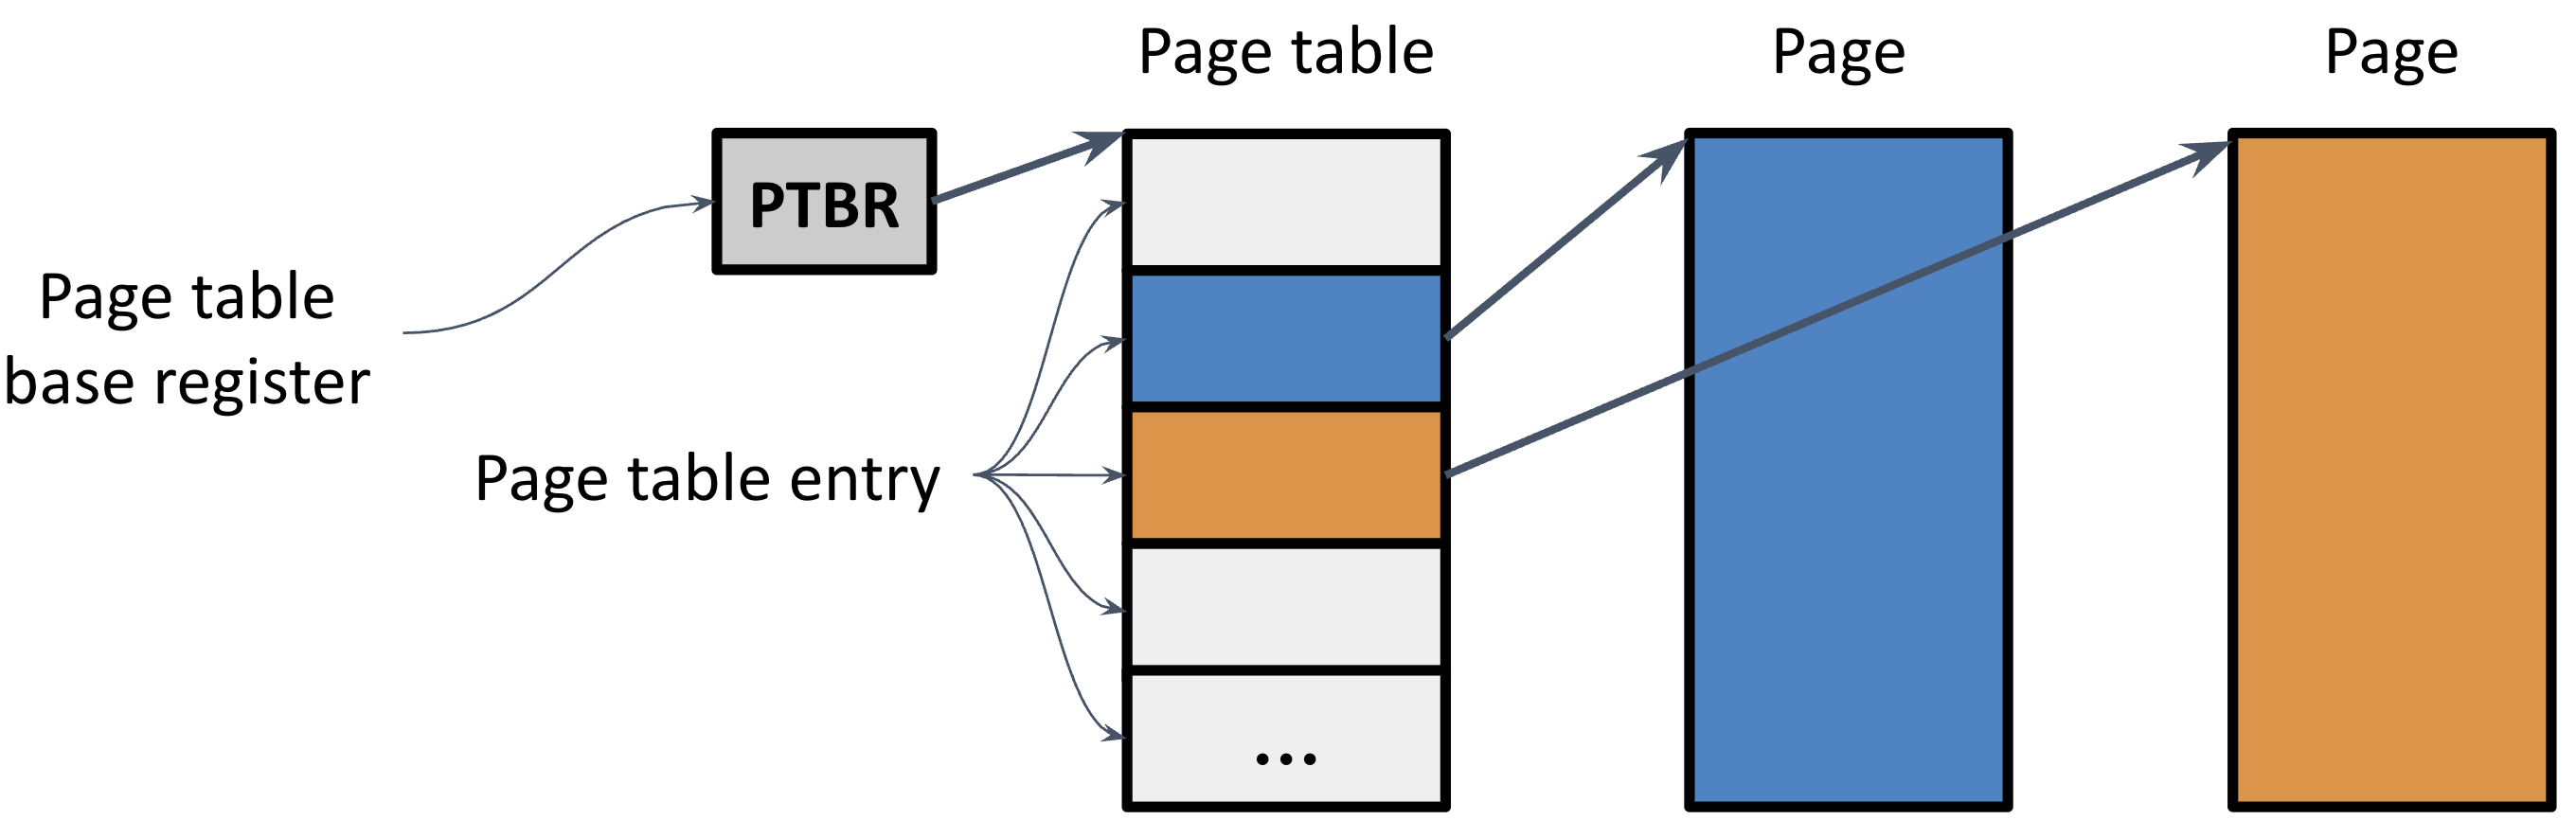
\includegraphics[width=0.55\textwidth]{chapters/L5/images/pte.png}
\end{center}

\begin{example}[Size of a Linear Page Table]
Consider the following assumptions:
\begin{itemize}
  \item[-] Virtual address size: 32 bits
  \item[-] Physical address size: 32 bits
  \item[-] Page size: 4 KB (i.e., 12 bits offset)
  \item[-] Each page table entry (PTE): 4 bytes
\end{itemize}

The size of the linear page table is calculated as follows:

\[
\text{Number of entries} = 2^{\text{Virtual Address Bits} - \text{Offset Bits}} = 2^{32 - 12} = 2^{20}
\]

Thus, the page table size is:

\[
\text{Page Table Size} = \text{Number of Entries} \times \text{Size per Entry} = 2^{20} \times 4\text{ bytes} = 4\text{ MiB}
\]
\end{example}
\vfill
\newpage
\subsection{Resolving addresses with a Linear Page Table (32-bit)}
In a 32-bit linear paging system, the address translation process from virtual to physical addresses follows a straightforward mechanism, detailed step-by-step below and illustrated bellow. 

\begin{enumerate}
    \item \textbf{Access Address Breakdown}
    \begin{itemize}
      \item[] The virtual (logical) address consists of two parts
        \begin{enumerate}
            \item \textbf{Page number} identifies the page in virtual memory.
            \item \textbf{Offset} identifies the byte within the page.
        \end{enumerate}
        For example, the address \texttt{20 983 809} can be split into:
        \begin{itemize}
            \item Page number \texttt{5123}
            \item Offset \texttt{1}
        \end{itemize}
    \end{itemize}

    \item \textbf{Lookup in Page Table}
    \begin{itemize}
        \item The Page Table Base Register (PTBR) points to the beginning of the page table in physical memory (in our example, \texttt{PTBR = 0x0}).
        \item The page number extracted from the virtual address (\texttt{5123}) is used as an index into the linear page table.
    \end{itemize}

    \item \textbf{Page Frame Identification} The entry at index \texttt{5123} in the page table provides the frame number in physical memory (in the diagram example, frame number \texttt{1026}).


    \item \textbf{Physical Address Computation}
    \begin{itemize}
        \item The physical frame number (\texttt{1026}) obtained from the page table and the original offset (\texttt{1}) from the virtual address are combined to form the physical address.
        \item This address directly maps to a unique location in physical memory.
    \end{itemize}

    \item \textbf{Accessing the Memory} Finally, the computed physical address is used to access the desired data in physical memory.
\end{enumerate}

\begin{center}
  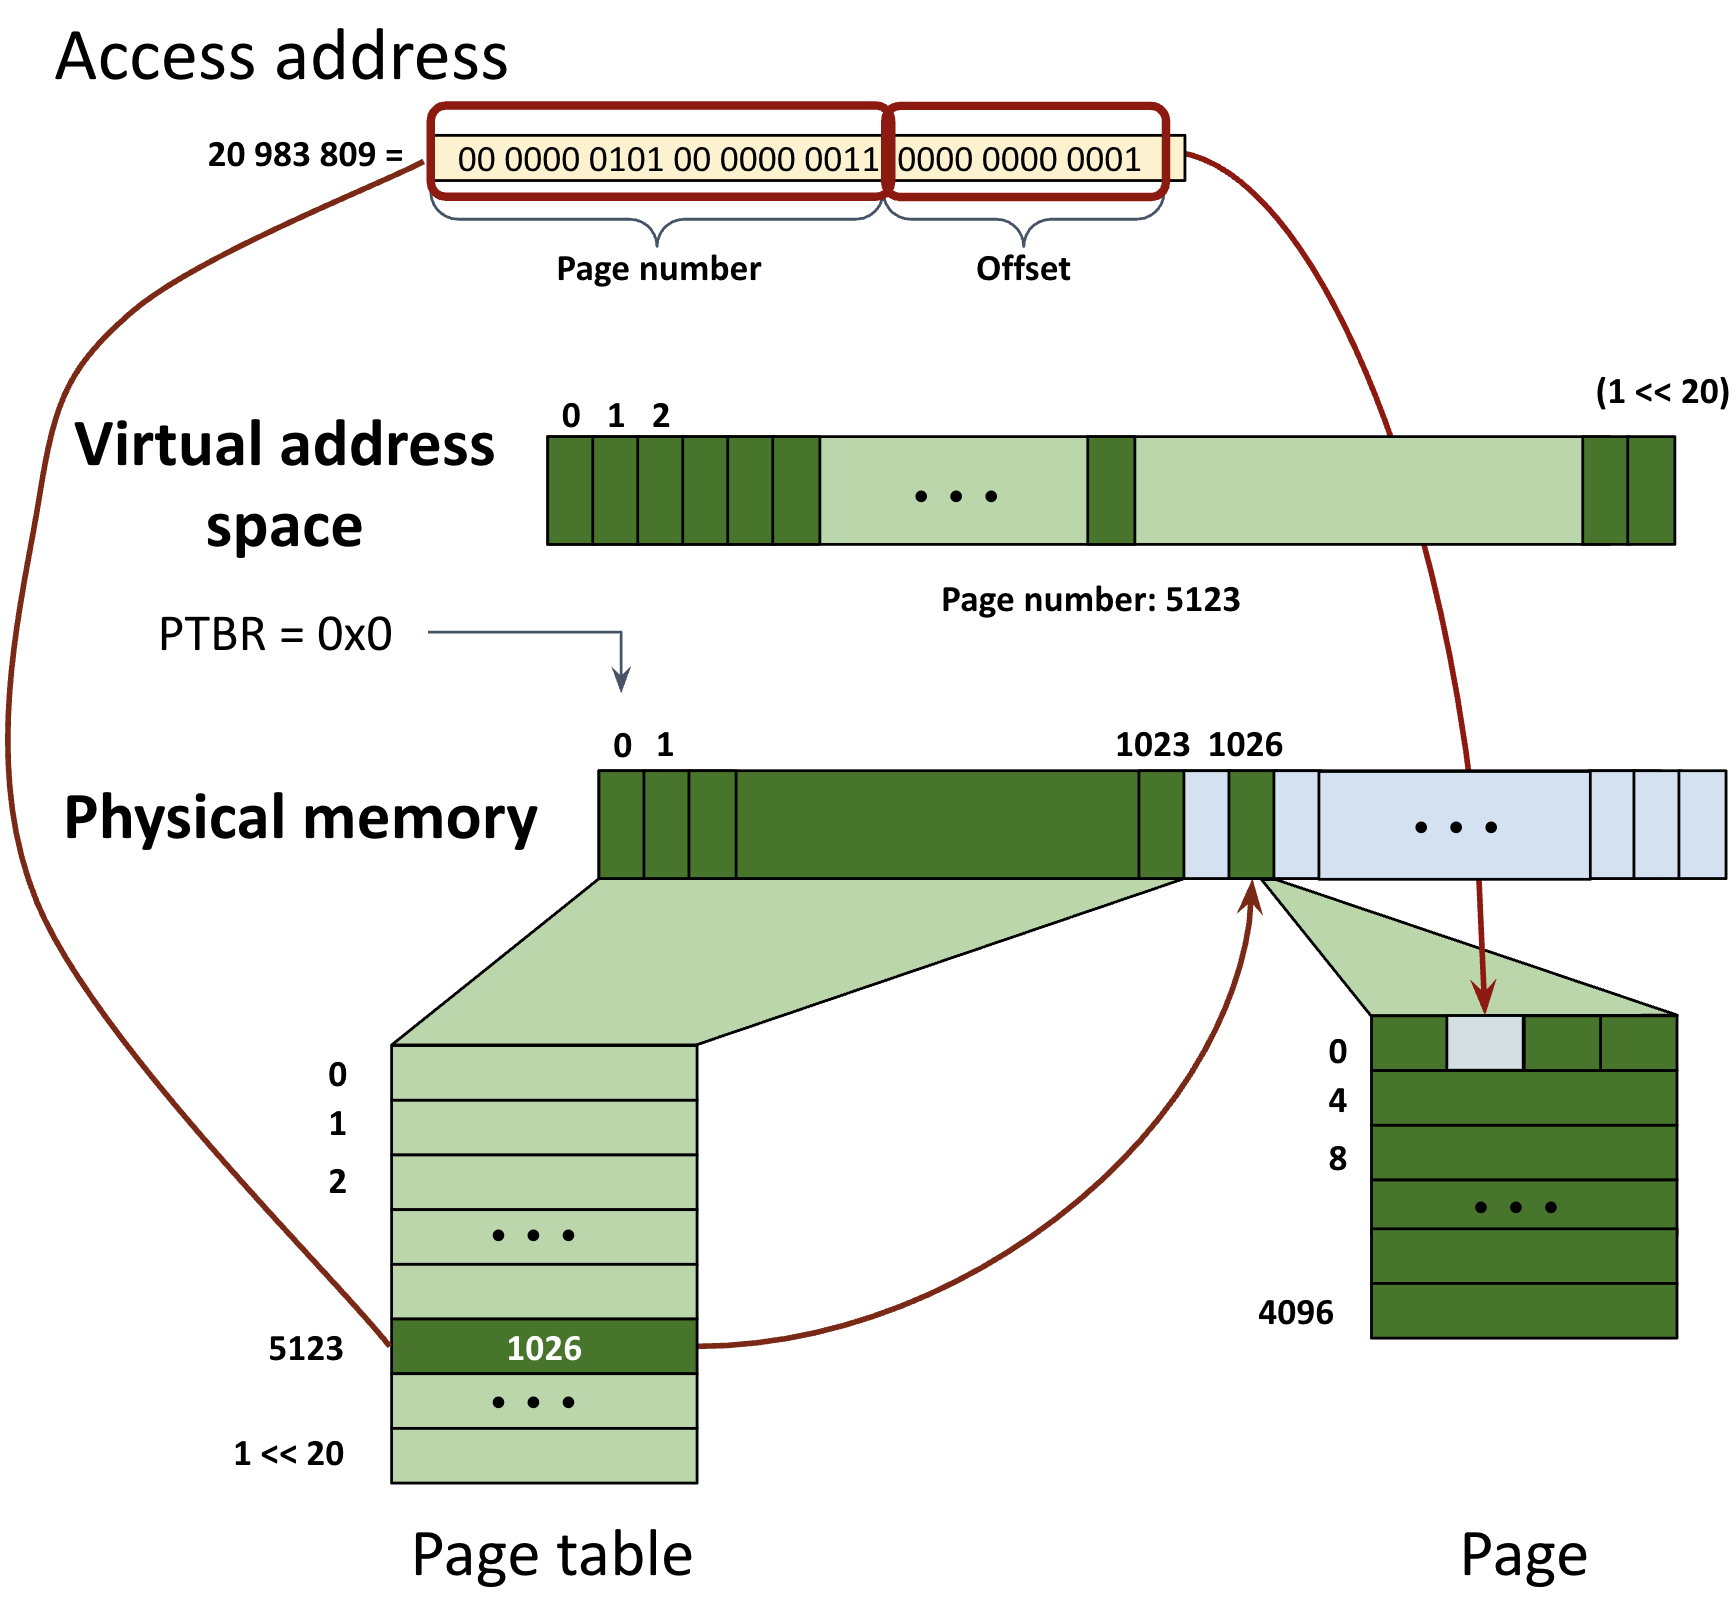
\includegraphics[width=0.65\textwidth]{chapters/L5/images/resolving.png}
\end{center}

This linear mapping approach is simple and direct but may require substantial memory for the page table, especially when handling large virtual address spaces, let's see how much.

\subsection{The Issue with Linear Page Tables (4 KB Pages)}

Using a linear page table with a 32-bit architecture, a 4 KB (12-bit offset) page size, and 4-byte entries results in a considerable memory overhead:
\[
\text{Number of entries} = 2^{32 - 12} = 2^{20}
\]
\[
\text{Page table size} = 2^{20} \times 4\,\text{bytes} = 4\,\text{MiB}
\]

Expanding this to 64-bit architectures significantly increases memory usage:

\begin{center}
\small
\begin{tabular}{|c|c|c|c|}
\hline
\textbf{Virtual Address Bits} & \textbf{Physical Address Bits} & \textbf{Entry Size} & \textbf{Page Table Size} \\
\hline
32 & 48 bit & 8 bytes & 8 MiB \\
64 & 64 bit & 8 bytes & $2^{52} \times 8$ bytes = 32 PiB \\
\hline
\end{tabular}
\end{center}
\normalsize
In 64-bit architectures with large, sparse address spaces, linear page tables quickly become impractical. Although increasing the page size (e.g., from \(16\,\mathrm{KiB}\) pages) can reduce memory overhead, it introduces significant internal fragmentation. Let's look at a more effective approach
\subsection{Multi-level Page Tables}
\small
Most processes use only a small fraction of the available address space. Multi-level page tables efficiently allocate metadata only for the used portion by organizing the page table in a hierarchy. Although each level adds an extra memory lookup during address translation, this method saves space overall. \\[5px]
\textbf{Analogy} Imagine locating a book in a library: first, you choose a section, then an aisle, then a shelf, and finally the book's position. \\[5px]
\textbf{Analogy 2  - This made me understand how multi-level paging is more memory efficient}\\
Imagine organizing a large library. \\[4px]
With a \textbf{linear (single-level) page table}, you'd have to create a catalog entry for \textit{every shelf}—even if most shelves are completely empty. This wastes space by reserving entries for unused shelves. \\[4px]
A \textbf{two-level page table} solves this problem by using a hierarchical catalog: the \textit{first-level catalog} only keeps track of sections of shelves that actually contain books. Detailed \textit{second-level catalogs} are created solely for these used sections, avoiding unnecessary records for empty shelves and significantly reducing memory usage.\\

\begin{example}[Two-Level Paging Example]
A virtual address on a 32-bit machine with a 4~KiB page size is divided as follows:
\begin{itemize}
  \item \textbf{Page offset:} 12 bits.
  \item \textbf{Page number:} 20 bits.
\end{itemize}
Since the page table is paged, the 20-bit page number is split into two 10-bit parts:
\begin{itemize}
  \item The first 10 bits index the first-level page table.
  \item The next 10 bits index the second-level page table.
\end{itemize}
With each page table entry occupying 4 bytes, a 4~KiB page can hold up to $\frac{4096}{4} = 1024 \quad (\text{or } 1 \ll 10) \quad \text{entries}$. \\
\noindent
\begin{minipage}{0.40\textwidth}
\begin{center}
  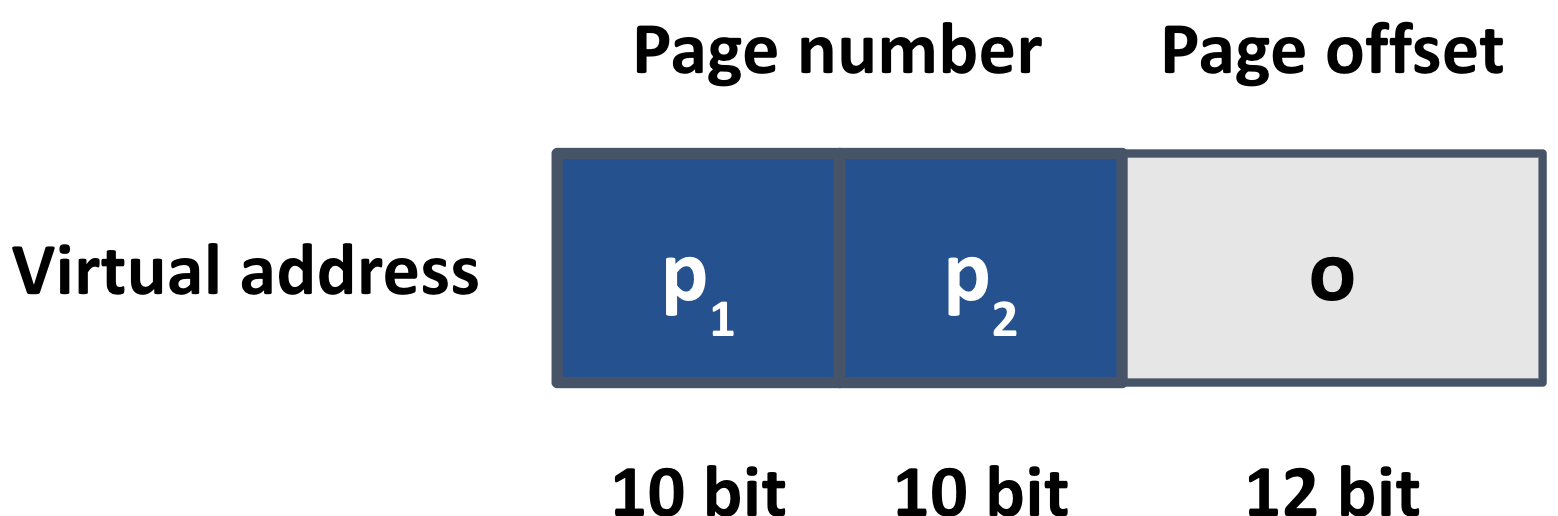
\includegraphics[width=0.9\textwidth]{chapters/L5/images/two-level-address.png}
\end{center}
\end{minipage}%
\hfill
\vline
\hfill
\begin{minipage}{0.50\textwidth}
\begin{center}
  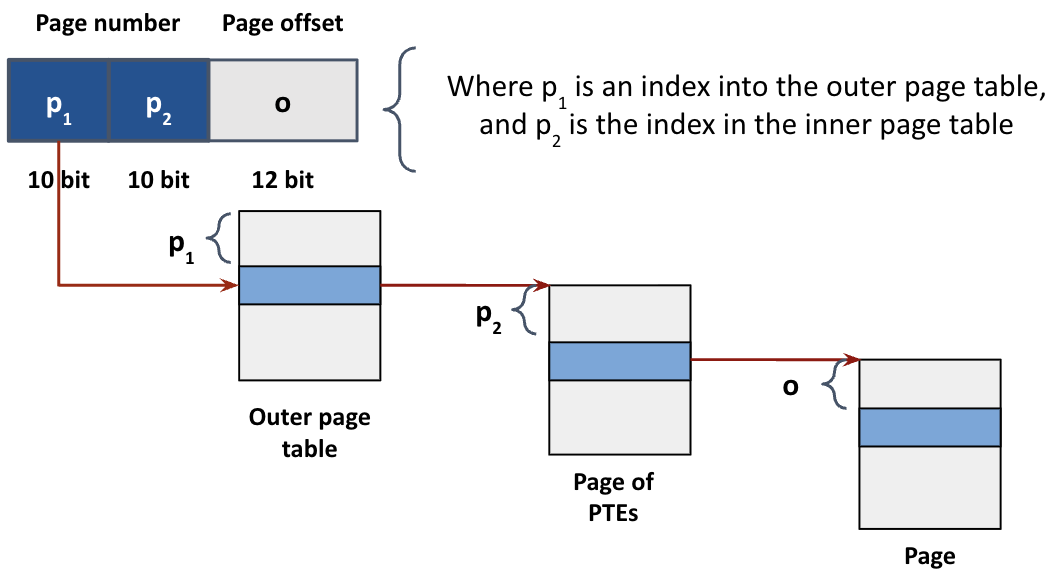
\includegraphics[width=1.1\textwidth]{chapters/L5/images/two-level-diagram.png}
\end{center}
\end{minipage}
\end{example}
\normalsize
\subsection{Resolving Addresses: Linear vs.\ Two-Level Paging (32-bit)}
\noindent
\begin{minipage}{0.42\textwidth}
\footnotesize
In a \emph{linear} (single-level) paging scheme for a 32-bit address space, the virtual address is typically split into two parts: 
\[
\underbrace{\text{Page Number}}_{20 \text{ bits}} \quad \underbrace{\text{Offset}}_{12 \text{ bits}}.
\]
The \emph{page number} serves as an index into a single page table, which holds the base address of the corresponding physical page. The \emph{offset} is then added to this base address to obtain the final physical address.

By contrast, in a \emph{two-level paging} scheme, the 20-bit page number is further subdivided into:
\[
\underbrace{\text{Page Directory Index}}_{10 \text{ bits}} 
\quad
\underbrace{\text{Page Table Index}}_{10 \text{ bits}}
\quad
\underbrace{\text{Offset}}_{12 \text{ bits}}.
\]
The top 10 bits (page directory index) point to an entry in the \emph{page directory}, which in turn identifies the base address of a particular \emph{page table}. The next 10 bits (page table index) select the entry in that page table, which gives the base address of the physical page. Finally, the offset is added to this base address to compute the physical address.\\[5px]
The main difference is that \emph{linear paging} uses a single, large page table for the entire virtual address space, whereas \emph{two-level paging} uses a hierarchy of smaller tables. 
\end{minipage}%
\hfill
\vline
\hfill
\begin{minipage}{0.55\textwidth}
  \begin{center}
    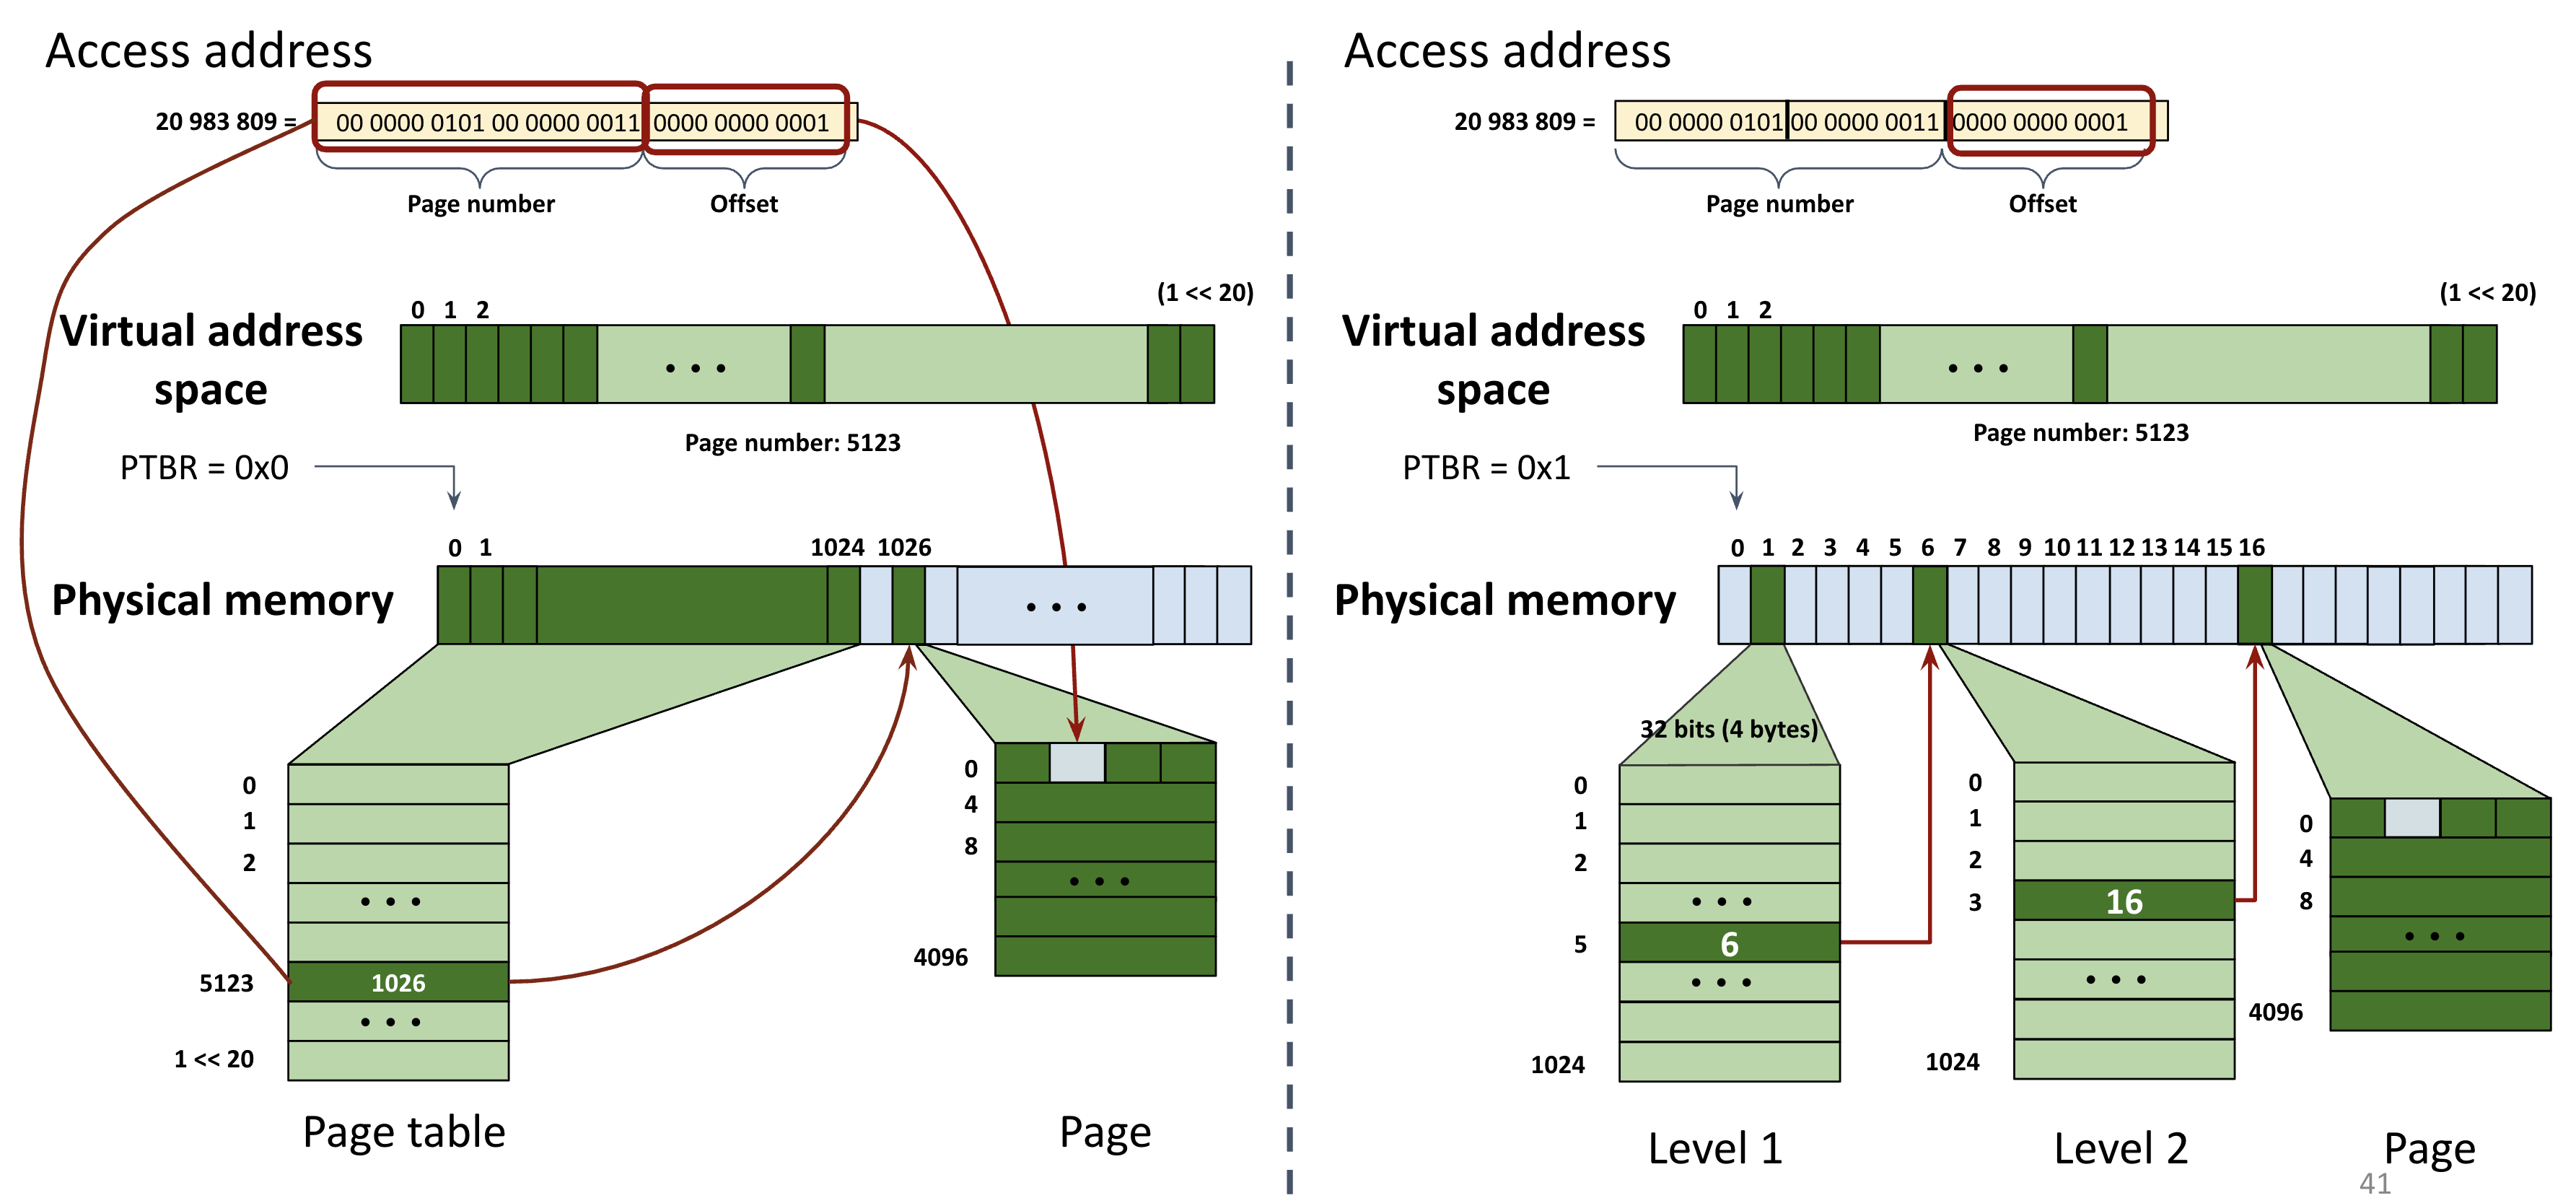
\includegraphics[width=1.2\textwidth]{chapters/L5/images/vs.png}
  \end{center}
\end{minipage}\\

\subsection{Multi-level Page Table for 64-bit Addressing}
In systems with a 4\,KiB page size (4096 bytes), each page holds 512 page table entries because 
\[
4096 \text{ bytes} \div 8 \text{ bytes/entry} = 512 \text{ entries} \quad (\text{requiring } 9 \text{ bits since } 2^9 = 512).
\]
For a full 64-bit address, subtracting the 12 bits used for the page offset leaves 52 bits to be mapped. A common scheme uses five levels of page tables for the first 45 bits (5 levels $\times$ 9 bits each) and a sixth level for the remaining 7 bits. If the virtual address space is reduced:
\begin{itemize}
  \item[-] To 57 bits: $57 - 12 = 45$ bits remain, which can be mapped with 5 levels.
  \item[-] To 48 bits: $48 - 12 = 36$ bits remain, requiring 4 levels.
\end{itemize}

\subsection{Paging: Advantages and Disadvantages}
\textbf{Advantages:}
\begin{itemize}
    \item \emph{No external fragmentation:} Memory is allocated in fixed-size pages.
    \item \emph{Fast allocation and deallocation:} Pages can be allocated or freed without searching for a contiguous memory block.
\end{itemize}

\textbf{Disadvantages:}
\begin{itemize}
    \item \emph{Memory overhead:} Additional space is required to store the page tables.
    \item \emph{Increased memory accesses:} Each memory access may require extra references to the page tables.
    \item \emph{Hardware complexity:} Efficient address translation demands specialized hardware (eg. we'll look at that hardware in the next section)
  \end{itemize}

\subsection{Logical Process of Memory Access in a Paging System}
When the CPU requests a code or data value at a virtual address, the following steps occur:
\begin{enumerate}
    \item The Memory Management Unit (MMU) begins a page table walk starting from the Page Table Base Register (PTBR).
    \item Depending on the address space:
    \begin{itemize}
      \item[-] A 32-bit address may require 2 memory references for translation.
      \item[-] A 48-bit address may require up to 4 memory references.
    \end{itemize}
    \item After the page table lookup, the page offset is added to the translated address to access the actual data in physical memory.
    \item To reduce the translation overhead, a cache called the Translation Lookaside Buffer (TLB) is used to store recent virtual-to-physical address mappings.
\end{enumerate}


\section{Translation Lookaside Buffer (TLB)}
\textit{Seen in a comparch, I'll try to make this clear.}\\

The Translation Lookaside Buffer (TLB) is a specialized, hardware-based cache that stores recent mappings from virtual addresses to physical addresses. When a process accesses memory, the Memory Management Unit (MMU) first checks the TLB:
\begin{itemize}
  \item[-] \textbf{TLB Hit:} If the mapping is present, the physical address is obtained directly, minimizing delay.
  \item[-] \textbf{TLB Miss:} If the mapping is absent, the MMU must perform a page table walk, involving multiple memory accesses, which is significantly slower.
\end{itemize}

The effectiveness of the TLB is largely due to the principle of locality of reference, which ensures a high hit rate under typical workloads. However, TLB entries can become invalid after a context switch or when page tables are updated.

\subsection{Memory Access Cost}
Assume a 64-bit address space and that all page table levels are cached when the TLB is present (i.e., on a TLB hit). The following table illustrates the number of memory accesses required to read or write a memory location \(X\) for a process:

\begin{center}
\begin{tabular}{l|c|c}
    \toprule
    \textbf{Page Table Level} & \textbf{With TLB \& TLB Hit} & \textbf{Without TLB} \\
    \midrule
    No Paging & 1 & 1 \\
    1 Level   & 1 & 2 \\
    2 Level   & 1 & 3 \\
    3 Level   & 1 & 4 \\
    \bottomrule
\end{tabular}
\end{center}

\textbf{Key:} The TLB is implemented as a dedicated circuit, separate from main memory, enabling rapid address translation.
\newpage
\subsection{TLB Lookup Process}
A Translation Lookaside Buffer (TLB) is a small, fast cache that stores recent virtual-to-physical address translations to speed up memory accesses. \\[9px]
\noindent
\begin{minipage}{0.45\textwidth}
\small
\begin{enumerate}
    \item \textbf{Decompose the virtual address:} 
    The processor splits the virtual address into two parts:
    \begin{itemize}
        \item \textit{Virtual Page Number (VPN)}: The high-order bits used for indexing or tagging in the TLB.
        \item \textit{Offset}: The low-order bits that remain unchanged when forming the physical address.
    \end{itemize}
    
    \item \textbf{Check the TLB:} The VPN is compared against the \emph{tag} fields of all TLB entries (often in parallel, if the TLB is fully associative). If a matching tag is found, it indicates a potential translation match.

    \item \textbf{Validate the match:}
    Along with the tag comparison, each TLB entry includes \emph{valid} and possibly other \emph{protection} bits. The processor checks these bits to ensure:
    \begin{itemize}
        \item The entry is valid (i.e., not stale or invalidated).
        \item The access permissions allow the requested operation (read, write, or execute).
    \end{itemize}
    If these checks pass, the match is confirmed.

    \item \textbf{Obtain the physical frame number (PFN):} Upon a valid match, the TLB entry provides the corresponding \emph{Physical Frame Number} (PFN). This is combined with the original offset to form the final physical address.

    \item \textbf{Handle TLB misses:}
    If no valid TLB entry matches the VPN (Virtual Page Number):
    \begin{itemize}
        \item The hardware (or the operating system, depending on the architecture) performs a \emph{page table walk} to locate the correct PFN in the page table.
        \item The discovered translation may then be loaded into the TLB for future accesses.
        \item The instruction or memory operation is retried with the updated TLB entry.
    \end{itemize}
\end{enumerate}
\end{minipage}%
\hfill
\vline
\hfill
\begin{minipage}{0.45\textwidth}
  \begin{center}
    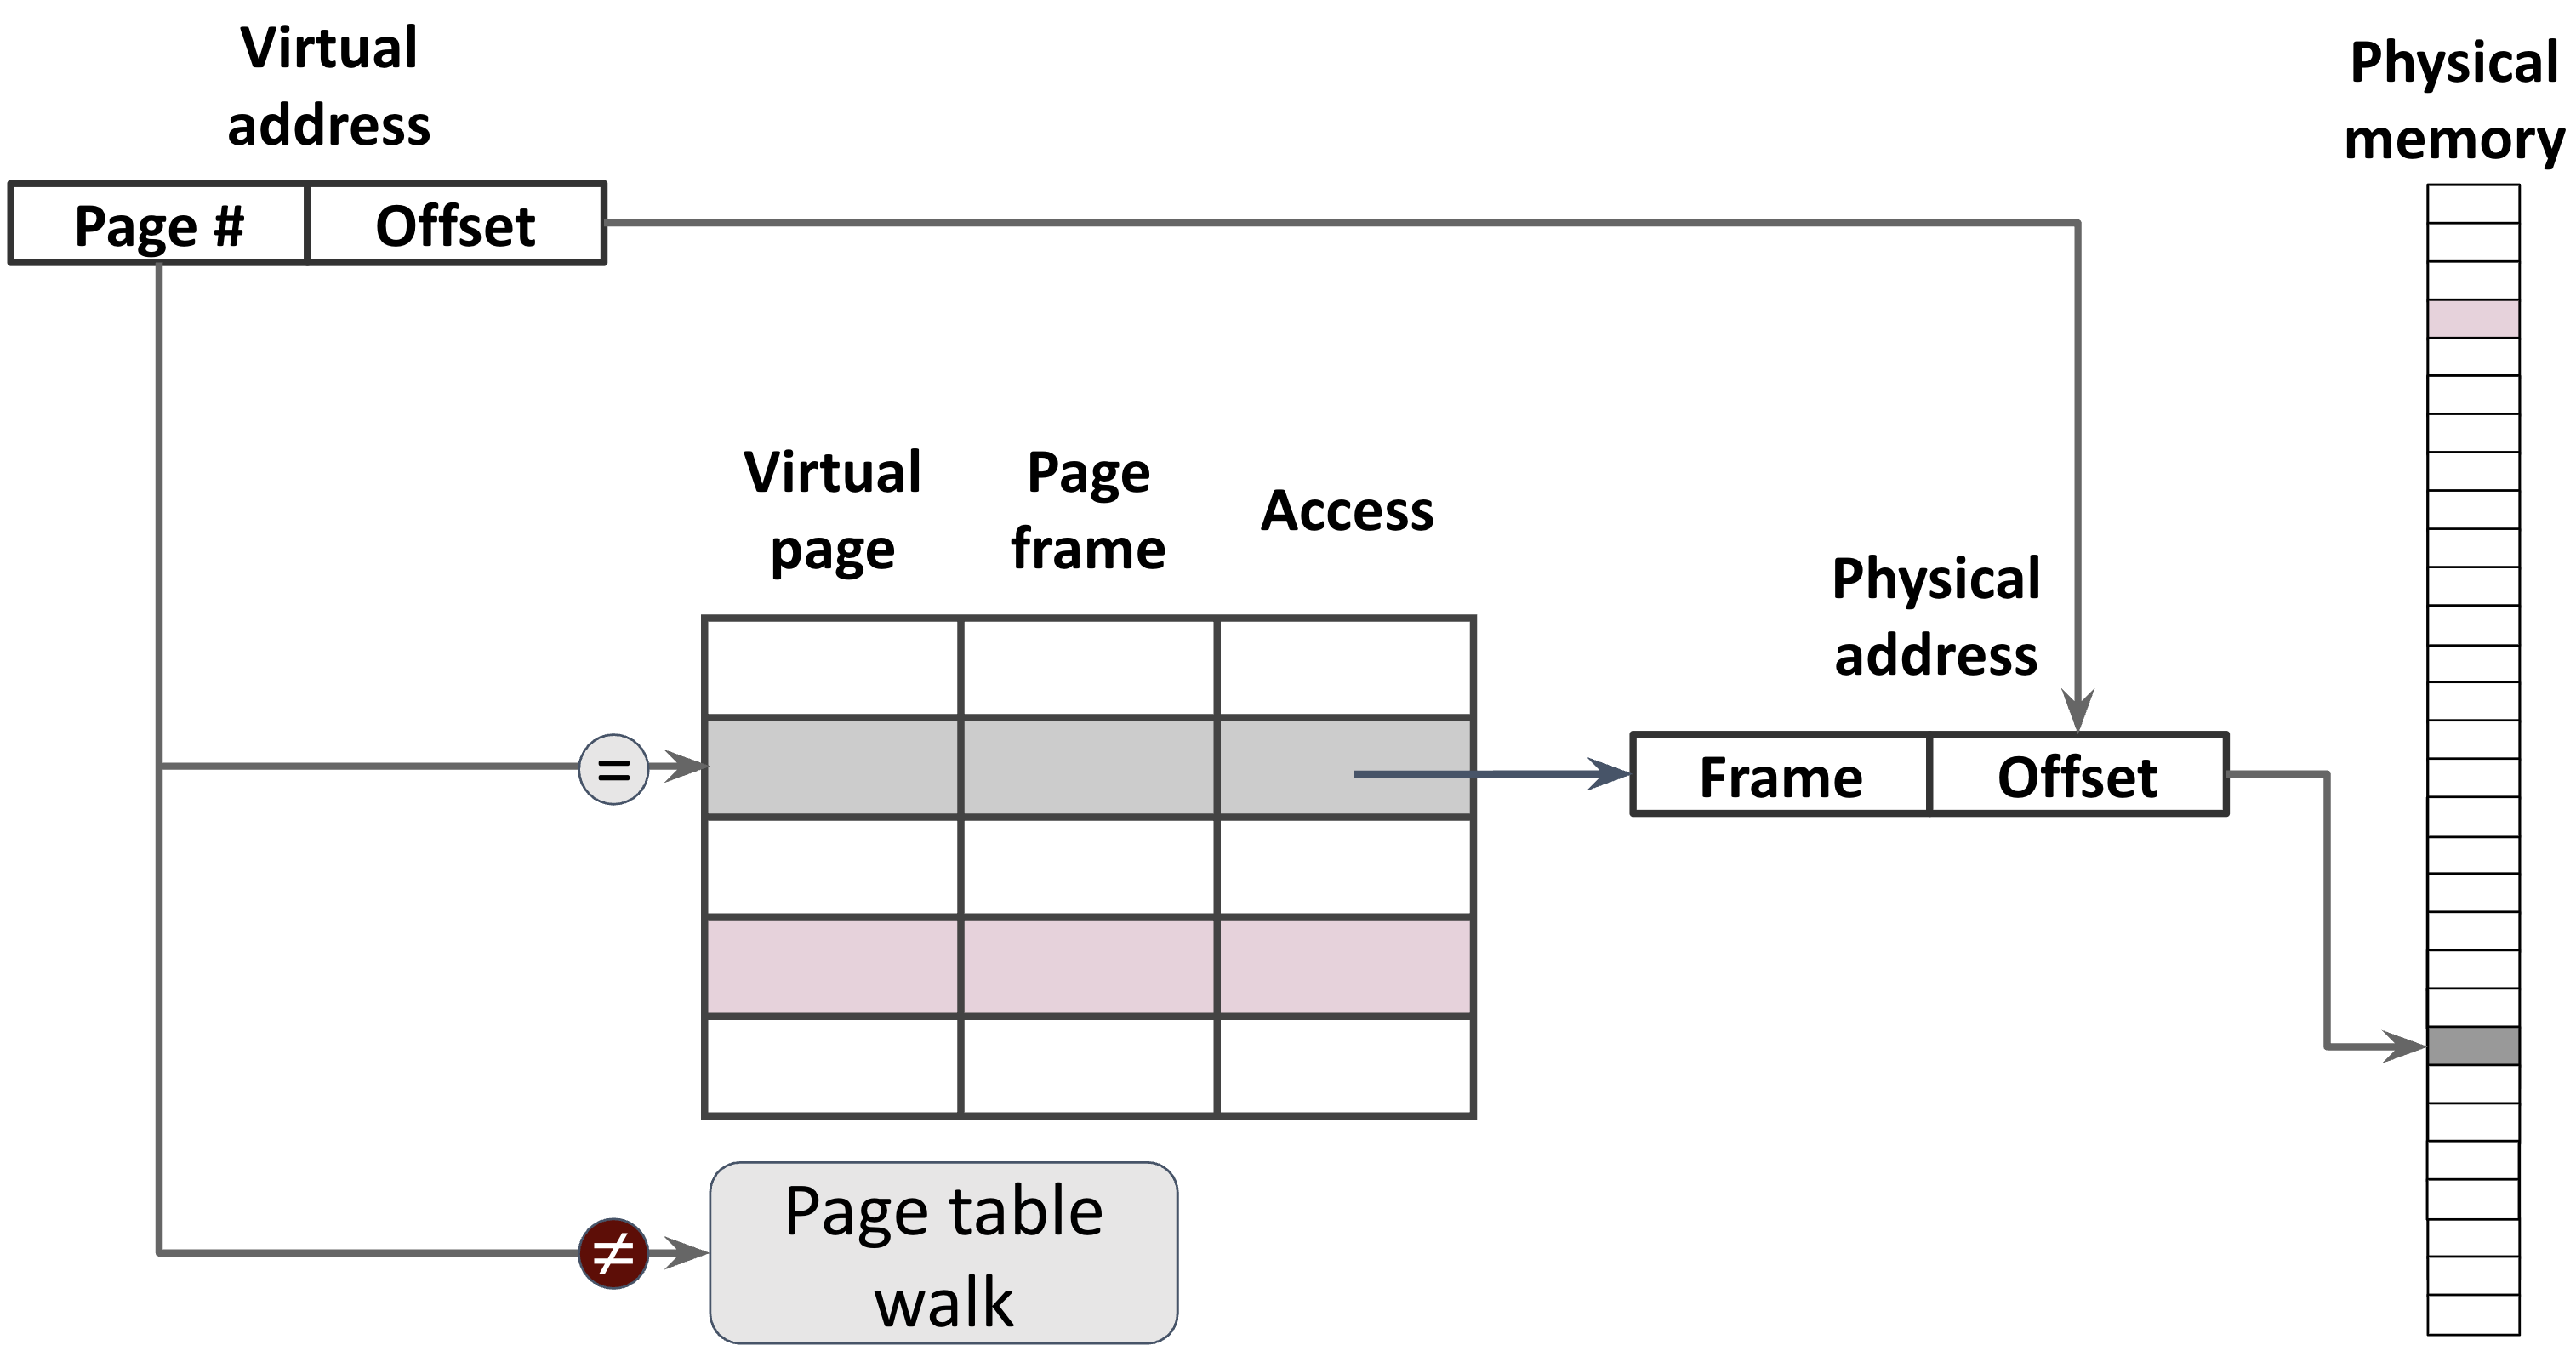
\includegraphics[width=1.25\textwidth]{chapters/L5/images/tlb.png}
  \end{center}
\end{minipage}\\[9px]

This process allows the CPU to translate virtual addresses into physical addresses quickly by leveraging the TLB's cached entries, significantly reducing the average memory access time.
\newpage
\subsection{CPU Execution of a Read/Write Operation}
\begin{enumerate}
    \item The CPU issues a load operation for a given virtual address (as part of a memory load/store).
    \item The Memory Management Unit (MMU) checks the Translation Lookaside Buffer (TLB) for the virtual address.
    \item \textbf{TLB Miss:}
    \begin{itemize}
        \item The MMU performs a page walk through the page table.
        \item If the Page Table Entry (PTE) is not present, a page fault occurs; the OS is invoked and a segmentation fault may be raised.
        \item If the PTE is present, the TLB is updated and execution continues.
    \end{itemize}
    \item \textbf{TLB Hit:} The physical address is obtained from the TLB, the memory location is fetched, and the data is returned to the CPU.
\end{enumerate}

\subsection{Summary: Page Tables}
\begin{itemize}
  \item[-] \textbf{Contents:} Page Table Entries (PTEs) that include permission bits.
  \item[-] \textbf{Size:} 
    \begin{itemize}
      \item[-] \textit{Linear Page Table:} Can be very large.
      \item[-] \textit{Multi-Level Page Table:} More memory efficient when sparsely populated.
    \end{itemize}
  \item[-] \textbf{Performance:} Paging overhead is mitigated by the use of the TLB.
  \item[-] \textbf{Memory Exhaustion:} Appropriate measures must be taken when the system runs out of memory.
\end{itemize}
\section{Swapping: Managing Memory Shortages}
When the physical memory is insufficient to hold all the active processes, the operating system (OS) employs a mechanism called \emph{swapping}. This process involves temporarily moving pages that are not actively used from main memory to disk storage. By doing so, the OS can reclaim memory for processes that require immediate attention and even over-provision memory beyond the available physical resources.

\subsection{Concepts}
\begin{itemize}
  \item[-] \textbf{Working Set:} The collection of pages a process actively uses at a given time. This set can change dynamically as the process executes.
  \item[-] \textbf{Storing Unused Pages:} By transferring inactive pages to disk, the OS frees up main memory for active processes.
  \item[-] \textbf{Over-Provisioning:} Swapping allows the system to allocate more virtual memory than is physically available.
\end{itemize}
\newpage
\subsection{Swapping In: Handling Page Faults}
When a process accesses a page that is not present in main memory, the Memory Management Unit (MMU) cannot translate the virtual address because the corresponding page table entry indicates that the page is absent. This situation results in a \emph{page fault}, prompting the OS to bring the page back from disk (swap-in).

\subsubsection{Page Fault Handling Procedure}
\begin{enumerate}
    \item \textbf{Address Translation:} The MMU translates virtual addresses to physical addresses using page tables. Each page table entry has a \textit{present bit} indicating if the page is in memory.
    \item \textbf{Page Fault Occurrence:} If the present bit is unset, a page fault is triggered.
    \item \textbf{Identifying the Fault:} The OS determines which process and address caused the fault by consulting its data structures.
    \item \textbf{Determining Page Status:}
    \begin{itemize}
        \item If the page is on disk, the OS issues a request to load it into memory.
        \item If the page has not been swapped out, the OS creates the mapping and updates its data structures.
    \end{itemize}
    \item \textbf{Context Switching:} While waiting for disk I/O, the OS may switch to another process.
    \item \textbf{Resuming Execution:} Once the page is loaded, the OS updates the page table entry and the Translation Lookaside Buffer (TLB), and then resumes the faulting process.
\end{enumerate}

\subsubsection{Swap-In Procedure}
\noindent
\begin{minipage}{0.45\textwidth}
\begin{enumerate}
    \item Locate the page in the swap cache.
    \item Allocate a new page in memory.
    \item Copy the content from disk to the allocated page.
    \item Update the page table entry to indicate that the page is now in memory.
    \item Load the corresponding TLB entry.
\end{enumerate}
\end{minipage}%
\hfill
\begin{minipage}{0.45\textwidth}
\begin{center}
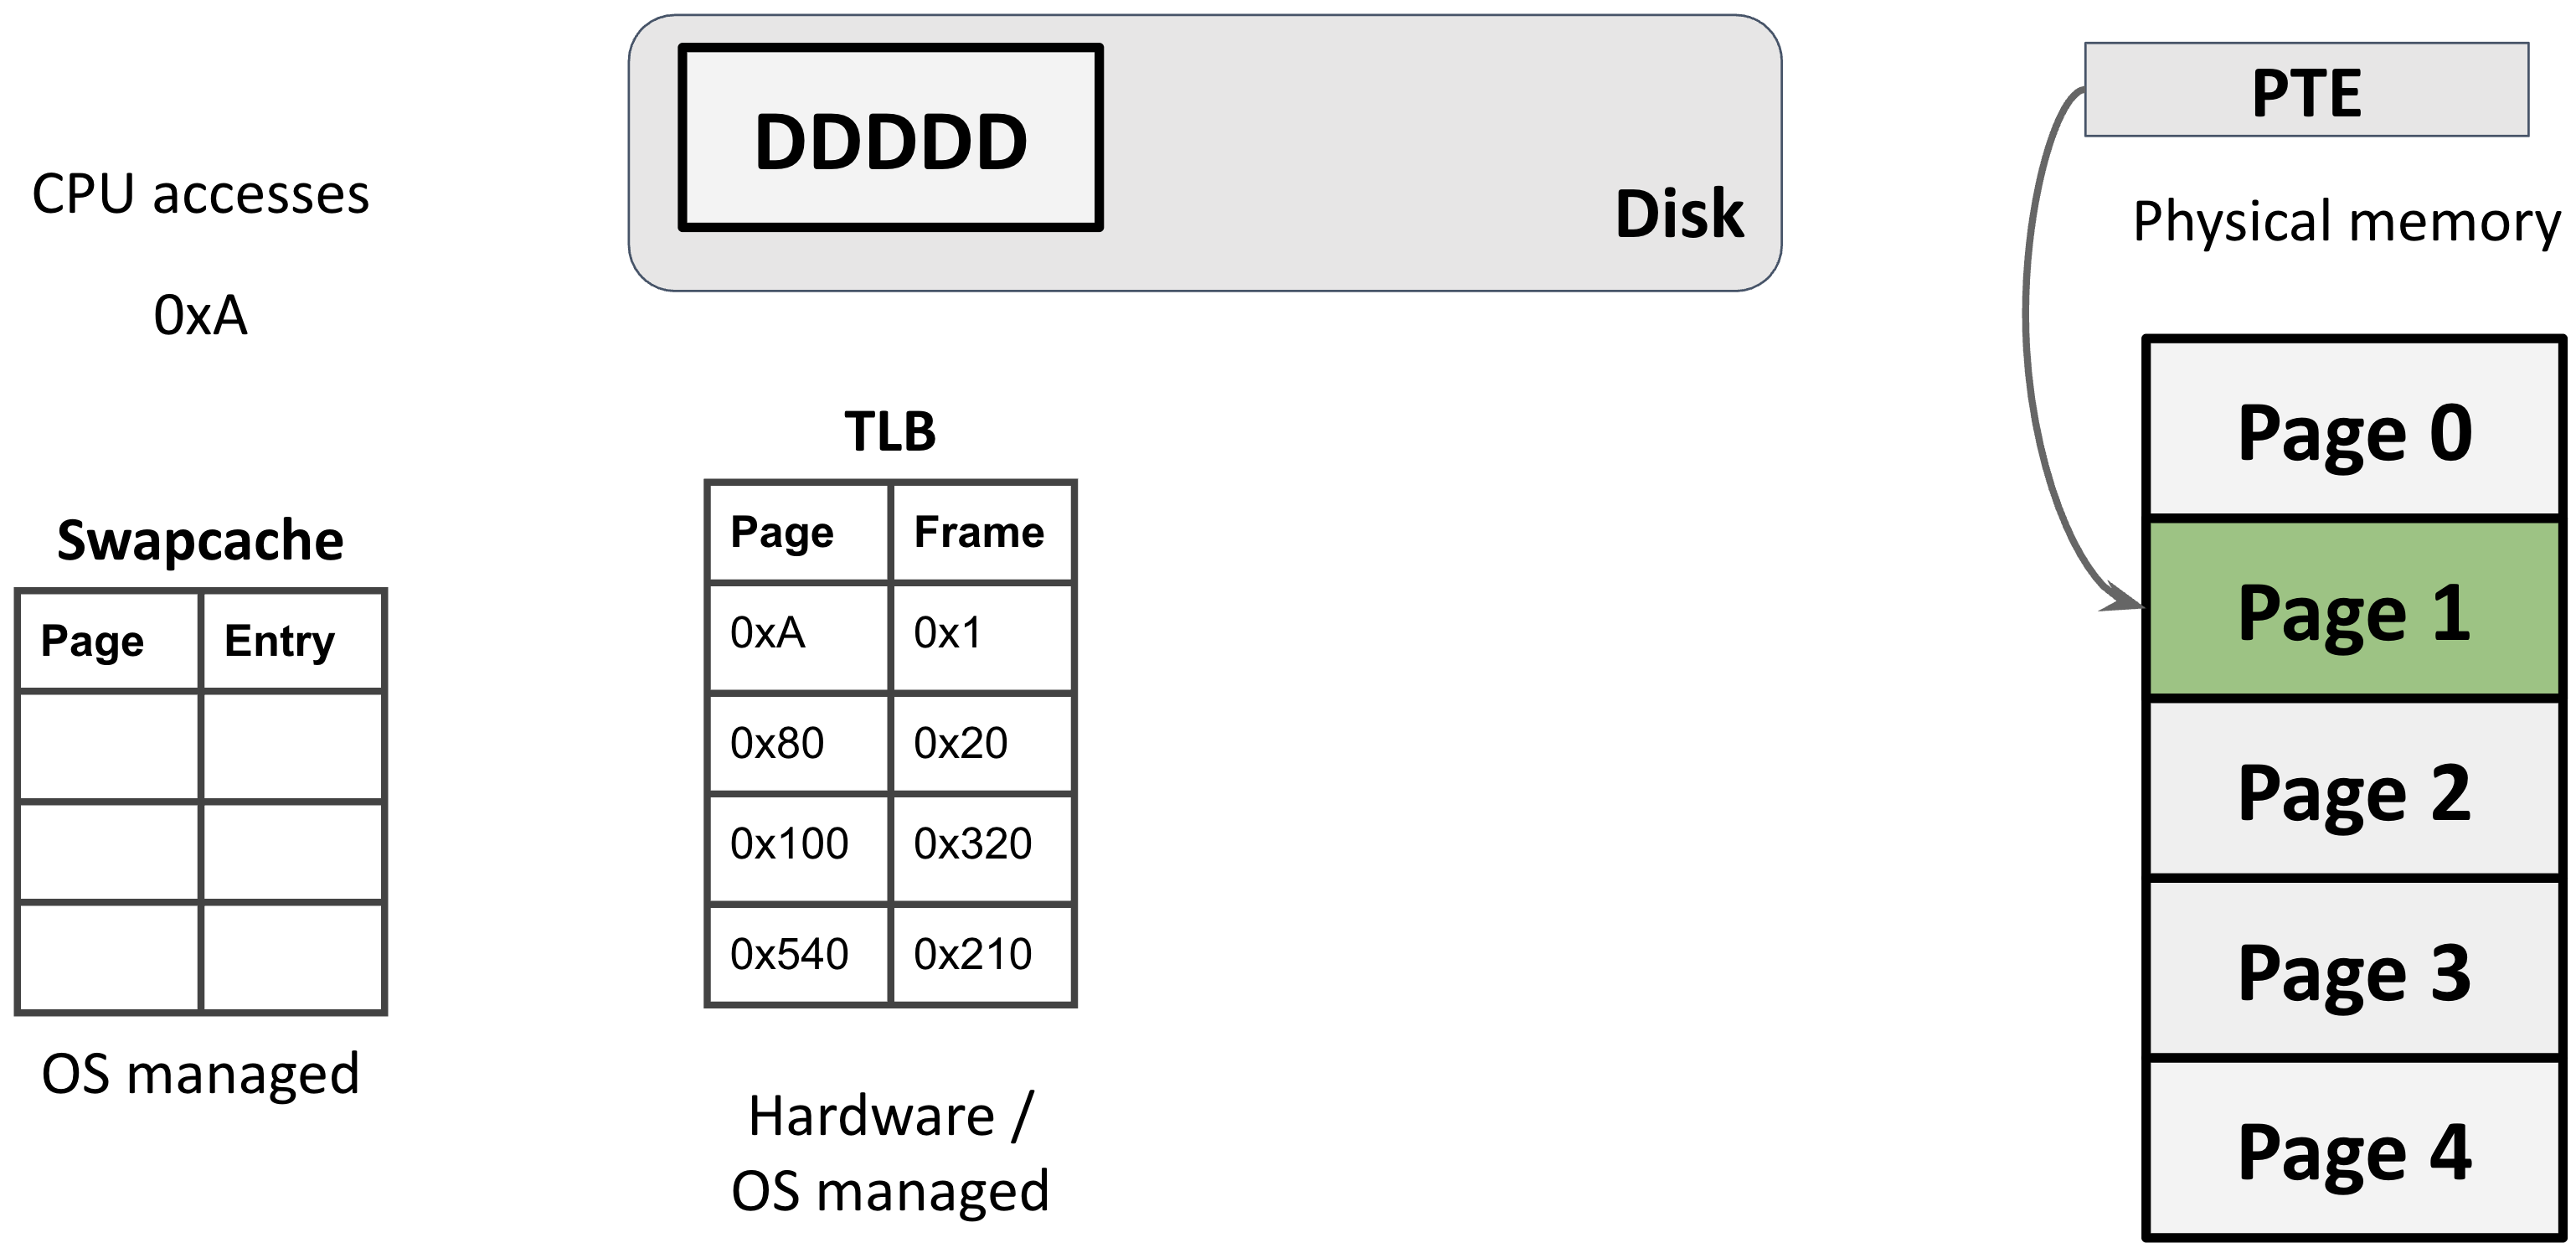
\includegraphics[width=1.1\textwidth]{chapters/L5/images/swapin.png}
\end{center}
\end{minipage}
\newpage
\subsection{Swapping Out: Freeing Up Memory}
Swapping out is the process of moving pages from main memory to disk, thereby freeing up physical memory for active processes. Although the steps involved are straightforward, choosing which pages to swap out is governed by complex OS policies to avoid performance degradation (e.g., thrashing).

\subsubsection{Swap-Out Procedure}
\noindent
\begin{minipage}{0.45\textwidth}
\begin{enumerate}
    \item Invalidate the corresponding TLB entry.
    \item Allocate an entry in the designated swap space.
    \item Copy the page content from memory to disk.
    \item Update the page table entry to reflect that the page is now stored on disk.
    \item Release the physical memory page.
\end{enumerate}
\end{minipage}%
\hfill
\begin{minipage}{0.45\textwidth}
\begin{center}
  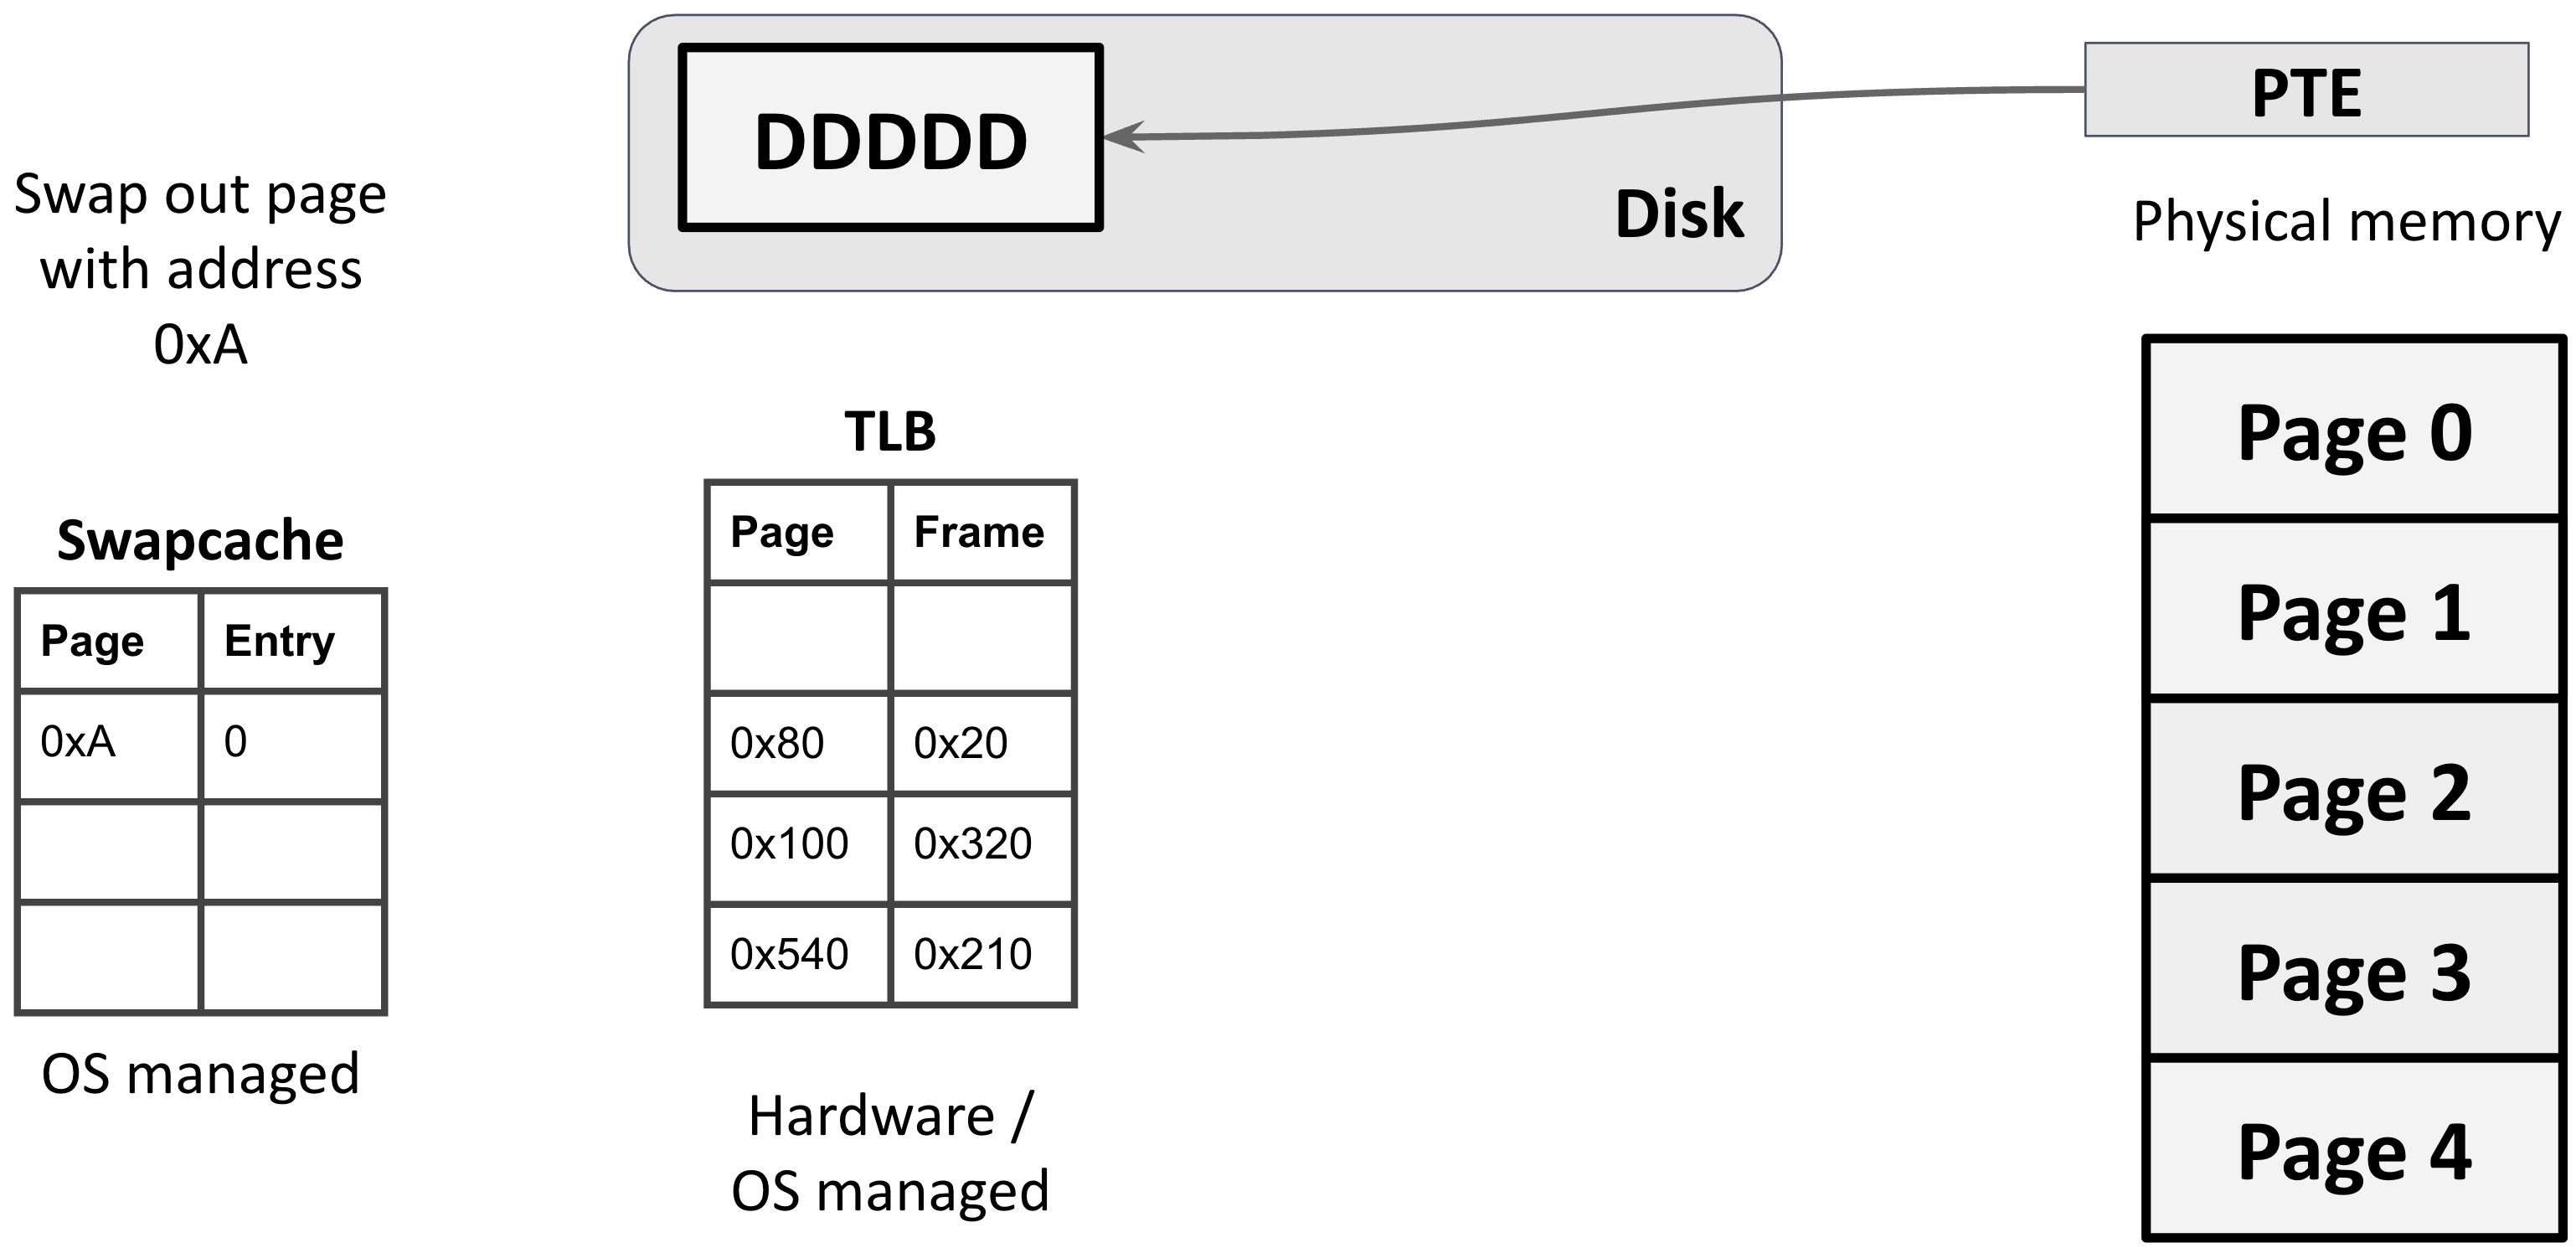
\includegraphics[width=1.1\textwidth]{chapters/L5/images/swapout.png}
\end{center}
\end{minipage}

\subsection{Conclusion}
Swapping is a vital mechanism in memory management, enabling the OS to manage limited physical memory efficiently by transferring inactive pages to disk. This dynamic exchange between main memory and disk ensures that active processes have the resources they need while also allowing the system to support a larger number of processes. However, careful policy decisions are essential to minimize overhead and avoid issues such as thrashing.
